\input{preamble}

% OK, start here.
%
\usepackage{fontspec}
\let\hyperwhite\relax
\let\hyperred\relax
\newcommand{\hyperwhite}{\hypersetup{citecolor=white,filecolor=white,linkcolor=white,urlcolor=white}}
\newcommand{\hyperred}{%
\hypersetup{%
    citecolor=TitlingRed,%
    filecolor=TitlingRed,%
    linkcolor=TitlingRed,%
     urlcolor=TitlingRed%
}}
\let\ChapterRef\relax
\newcommand{\ChapterRef}[2]{#1}
\setcounter{tocdepth}{2}
%▓▓▓▓▓▓▓▓▓▓▓▓▓▓▓▓▓▓▓▓▓▓▓▓▓▓▓▓▓▓▓▓▓
%▓▓ ╔╦╗╦╔╦╗╦  ╔═╗  ╔═╗╔═╗╔╗╔╔╦╗ ▓▓
%▓▓  ║ ║ ║ ║  ║╣   ╠╣ ║ ║║║║ ║  ▓▓
%▓▓  ╩ ╩ ╩ ╩═╝╚═╝  ╚  ╚═╝╝╚╝ ╩  ▓▓
%▓▓▓▓▓▓▓▓▓▓▓▓▓▓▓▓▓▓▓▓▓▓▓▓▓▓▓▓▓▓▓▓▓
%\usepackage{titlesec}
%▓▓▓▓▓▓▓▓▓▓▓▓▓▓▓▓▓▓▓▓▓▓▓▓▓▓▓▓▓▓▓▓▓▓▓▓▓▓▓▓▓▓▓▓▓▓▓▓▓▓▓▓▓▓▓
%▓▓ ╔╦╗╔═╗╔╗ ╦  ╔═╗  ╔═╗╔═╗  ╔═╗╔═╗╔╗╔╔╦╗╔═╗╔╗╔╔╦╗╔═╗ ▓▓
%▓▓  ║ ╠═╣╠╩╗║  ║╣   ║ ║╠╣   ║  ║ ║║║║ ║ ║╣ ║║║ ║ ╚═╗ ▓▓
%▓▓  ╩ ╩ ╩╚═╝╩═╝╚═╝  ╚═╝╚    ╚═╝╚═╝╝╚╝ ╩ ╚═╝╝╚╝ ╩ ╚═╝ ▓▓
%▓▓▓▓▓▓▓▓▓▓▓▓▓▓▓▓▓▓▓▓▓▓▓▓▓▓▓▓▓▓▓▓▓▓▓▓▓▓▓▓▓▓▓▓▓▓▓▓▓▓▓▓▓▓▓
\newcommand{\ChapterTableOfContents}{%
    \begingroup
    \addfontfeature{Numbers={Lining,Monospaced}}
    \hypersetup{hidelinks}\tableofcontents%
    \endgroup
}%

\let\DotFill\relax
\makeatletter
\newcommand \DotFill {\leavevmode \cleaders \hb@xt@ .33em{\hss .\hss }\hfill \kern \z@}
\makeatother

\definecolor{ToCGrey}{rgb}{0.4,0.4,0.4}
\definecolor{mainColor}{rgb}{0.82745098,0.18431373,0.18431373}
\usepackage{titletoc}
\titlecontents{part}
[0.0em]
{\addvspace{1pc}\color{TitlingRed}\large\bfseries\text{Part }}
{\bfseries\textcolor{TitlingRed}{\contentslabel{0.0em}}\hspace*{1.35em}}
{}
{\textcolor{TitlingRed}{{\hfill\bfseries\contentspage\nobreak}}}
[]
\titlecontents{section}
[0.0em]
{\addvspace{1pc}}
{\color{black}\bfseries\textcolor{TitlingRed}{\contentslabel{0.0em}}\hspace*{1.65em}}
{}
{\textcolor{black}{\textbf{\DotFill}{\bfseries\contentspage\nobreak}}}
[]
\titlecontents{subsection}
[0.0em]
{}
{\hspace*{1.65em}\color{ToCGrey}{\contentslabel{0.0em}}\hspace*{2.5em}}
{}
{{\textcolor{ToCGrey}\DotFill}\textcolor{ToCGrey}{\contentspage}\nobreak}
[]
\usepackage{marginnote}
\renewcommand*{\marginfont}{\normalfont}
\usepackage{inconsolata}
\setmonofont{inconsolata}%
\let\ChapterRef\relax
\newcommand{\ChapterRef}[2]{#1}
\AtBeginEnvironment{subappendices}{%%
    \section*{\huge Appendices}%
}%

\begin{document}

\title{Real Analysis}

\maketitle

\phantomsection
\label{section-phantom}

This chapter contains material on real analysis.

\ChapterTableOfContents

TODO copy pasted from email:
\begin{enumerate}
    \item \url{https://link.springer.com/book/10.1007/978-3-030-43788-6}
    \item \url{https://math.mit.edu/classes/18.095/2015IAP/lecture1/padic.pdf}
    \item \url{https://golem.ph.utexas.edu/category/2023/09/constructing_the_real_numbers.html}
    \item \url{https://andrescaicedo.wordpress.com/wp-content/uploads/2014/09/ross-street-an-efficient-construction-of-real-numbers.pdf}
    \item \url{https://mathoverflow.net/questions/401441/a-natural-construction-of-real-numbers}
    \item \url{https://mathoverflow.net/questions/310466/eudoxus-real-numbers?rq=1}
    \item \url{https://arxiv.org/abs/math/0301015v1}
    \item \url{https://www.maths.mq.edu.au/~street/reals.pdf}
    \item \url{https://mathoverflow.net/questions/339348/the-real-numbers-as-a-wreath-product?rq=1}
    \item \url{https://www.universiteitleiden.nl/binaries/content/assets/science/mi/scripties/bachelor/2017-2018/hermans-bscthesis.pdf}
    \item \url{https://science.mq.edu.au/~street/EffR.pdf}
    \item \url{https://arxiv.org/abs/1306.2382}
    \item \url{https://repository.lsu.edu/josa/vol5/iss2/3/}
    \item \url{https://math.stackexchange.com/questions/3652852/how-does-conways-proposed-compromise-for-constructing-the-real-numbers-actually}
    \item \url{https://www.youtube.com/watch?v=mPn2AdMH7UQ}
    \item \url{https://www.youtube.com/watch?v=elVQtF6T5Zk}
    \item \url{https://www.youtube.com/watch?v=9-nerkgryZ8}
    \item \url{https://plato.stanford.edu/entries/infinity/surreal-numbers.html}
    \item \url{https://www.m-a.org.uk/resources/downloads/4H-Jim-Simons-Meet-the-surreal-numbers.pdf}
    \item \url{https://medium.com/badiou-and-science/badiou-and-science-1-4-1-the-surreal-numbers-part-1-95dadcf4c554}
    \item \url{https://mathoverflow.net/questions/63320/where-do-surreal-numbers-come-from-and-what-do-they-mean}
    \item \url{https://core.ac.uk/download/pdf/76357132.pdf}
    \item \url{https://perso.eleves.ens-rennes.fr/people/clementine.laurens/Documents\%20page\%20web\%20perso/ENS\%20Rennes/Stage\%20L3/Rapport\%20de\%20stage\%20L3\%20-\%20Conway\%27s\%20numbers.pdf}
    \item \url{https://web.mit.edu/sp.268/www/2010/surreal.pdf}
    \item \url{https://mathoverflow.net/questions/418403/a-surnatural-numbers-as-a-largest-model-of-the-natural-numbers}
    \item \url{http://www.goodmath.org/blog/2007/03/29/introducing-the-surreal-numbers-edited-rerun/}
    \item \url{https://guests.mpim-bonn.mpg.de/spc/teaching/numbers_1617/}
    \item \url{https://w3.impa.br/~goncalves/avitalslides.pdf}
    \item \url{https://guests.mpim-bonn.mpg.de/spc/talks/7_gandalf_surrealnumbers_notes.pdf}
    \item \url{https://www.infinitelymore.xyz/p/surreal-numbers}
    \item \url{https://www.whitman.edu/Documents/Academics/Mathematics/Grimm.pdf}
    \item \url{https://math.stackexchange.com/questions/4482314/can-the-surreal-numbers-be-completed-to-form-an-ordered-field}
    \item \url{https://en.wikipedia.org/wiki/Surreal_number}
    \item \url{https://en.wikipedia.org/wiki/Superreal_number}
    \item \url{https://en.wikipedia.org/wiki/Levi-Civita_field}
    \item \url{https://en.wikipedia.org/wiki/Hyperreal_number}
    \item \url{https://mathoverflow.net/questions/478411/can-the-canonical-eudoxus-real-representatives-be-defined-easily}
    \item \url{https://www.google.com/search?client=firefox-b-d&q=construction+of+the+real+numbers+from+hyperreal+numbers}
    \item \url{https://estudogeral.uc.pt/bitstream/10316/89416/1/ordgrp\%20JPAA.pdf}
    \item \url{https://arxiv.org/abs/2212.07064}
    \item \url{https://arxiv.org/pdf/2005.07738}
    \item \url{https://arxiv.org/pdf/2406.10071v1}
    \item \url{https://www.youtube.com/watch?v=f8CXG7dS-D0}
    \item \url{https://www.youtube.com/watch?v=tR1HTNtcYw0}
    \item \url{https://www.youtube.com/watch?v=NAREJqDQb_U}
    \item \url{https://www.youtube.com/watch?v=TvWJPMfkVJg}
\end{enumerate}
TODO:
\begin{enumerate}
    \item An Integer Construction of Infinitesimals: Toward a Theory of Eudoxus Hyperreals
    \item The Eudoxus reals constructed in homotopy type theory, \url{https://pure.tue.nl/ws/portalfiles/portal/175415888/Fokma_A..pdf}
    \item \url{https://golem.ph.utexas.edu/category/2023/09/constructing_the_real_numbers.html}
    \item \url{https://www.isa-afp.org/browser_info/current/AFP/Eudoxus_Reals/outline.pdf}
    \item \url{https://arxiv.org/pdf/2310.04534}
    \item \url{https://mattbaker.blog/2021/12/15/the-eudoxus-reals/}
    \item \url{https://link.springer.com/article/10.1007/s00013-005-1413-z}
    \item \url{https://github.com/Lix0120/eudoxus}
    \item \url{https://arxiv.org/abs/math/0301015v1}
    \item \url{https://arxiv.org/abs/math/0405454v1}
    \item Is there a relation between the paracyclic category and the Eudoxus real numbers?
    \item Construction of $\R$ from hyperreal numbers, \url{https://en.wikipedia.org/wiki/Construction_of_the_real_numbers#Construction_using_hyperreal_numbers}
    \item Construction of $\R$ from surreal numbers, \url{https://en.wikipedia.org/wiki/Construction_of_the_real_numbers#Construction_from_surreal_numbers}
    \item Constructions of the $p$-adic numbers
        \begin{enumerate}
            \item Via Cauchy sequences
            \item Via filters
            \item Via Eudoxus
        \end{enumerate}
    \item \url{https://mathoverflow.net/questions/476939/how-to-define-dedekind-reals-and-eudoxus-reals-such-that-they-are-equivalent-to}
\end{enumerate}
TODO general analysis things:
\begin{enumerate}
    \item \url{https://en.wikipedia.org/wiki/Schwarzian_derivative}
    \item $L^p$ spaces but they take values in fields other than R or C
    \item Holder and minkowsky inequalities for $0\less p\less 1$
    \item topological vector spaces in characteristic p
    \item \url{https://mathoverflow.net/questions/66332/is-the-characteristic-of-a-field-detectable-from-the-topology-of-a-topological-v}
    \item \url{https://en.m.wikipedia.org/wiki/Stochastic_analysis_on_manifolds}
        \begin{quote}
            Stochastic differential geometry provides insight into classical analytic problems, and offers new approaches to prove results by means of probability. For example, one can apply Brownian motion to the Dirichlet problem at infinity for Cartan-Hadamard manifolds[4] or give a probabilistic proof of the Atiyah-Singer index theorem.
        \end{quote}
    \item Information theory and information geometry Wikipedia pages
    \item Inverse of Radon nykodim derivative
    \item derivative is not continuous as a morphism of normed spaces but works with sobolev norm
    \item Gohberg--Krein theorem as a generalisation of Riesz--Kakutani or something
    \item \url{https://en.wikipedia.org/wiki/Singular_integral}
    \item \url{https://en.wikipedia.org/wiki/Singular_integral_operators_of_convolution_type}
    \item Interpolation theory
        \begin{enumerate}
            \item \url{https://en.wikipedia.org/wiki/Interpolation_space}
            \item \url{https://link.springer.com/book/10.1007/978-88-7642-638-4}
            \item \url{https://www.math.cmu.edu/~iantice/notes/interpolation_notes.pdf}
        \end{enumerate}
    \item \url{https://en.wikipedia.org/wiki/Hardy\%E2\%80\%93Littlewood_maximal_function}
    \item \url{https://en.wikipedia.org/wiki/Calder\%C3\%B3n\%E2\%80\%93Zygmund_lemma}
    \item \url{https://markkm.com/pdf/MaximalFunctionTheory.pdf}
    \item \url{https://en.wikipedia.org/wiki/Jordan_operator_algebra}
    \item Fractional analysis
        \begin{enumerate}
            \item \url{https://en.wikipedia.org/wiki/Riesz_potential}
            \item \url{https://mathoverflow.net/a/292882}
            \item \url{https://en.wikipedia.org/wiki/Fractional_Laplacian}
            \item \url{https://arxiv.org/abs/1801.09767}
            \item \url{https://mathoverflow.net/a/292904/130058}
            \item \url{https://mathoverflow.net/questions/21929/what-is-the-actual-meaning-of-a-fractional-derivative#comment564388_228528}
            \item \url{https://mathoverflow.net/a/245061/130058}
            \item \url{https://mathoverflow.net/questions/21929/what-is-the-actual-meaning-of-a-fractional-derivative}
        \end{enumerate}
    \item Product integration
        \begin{enumerate}
            \item \url{https://en.wikipedia.org/wiki/Ordered_exponential}
        \end{enumerate}
\end{enumerate}

\section{Constructions of the Real Numbers}\label{section-constructions-of-the-real-numbers}
\subsection{The Dedekind Real Numbers}\label{subsection-the-dedekind-real-numbers}
\begin{definition}{Dedekind Cuts}{dedekind-cuts}%
    A \index[real-analysis]{Dedekind cut}\textbf{Dedekind cut} is a pair $(A,B)$ with $A,B\subset\Q$ satisfying the following conditions:
    \begin{enumerate}
        \item\label{dedekind-cuts-1}\SloganFont{Nonemptiness. }We have $A\neq\emptyset$.
        \item\label{dedekind-cuts-2}\SloganFont{Properness. }We have $A\neq\Q$.
        \item\label{dedekind-cuts-3}\SloganFont{Downward-Closedness. }For each $x,y\in\Q$, if $x\leq y$ and $y\in A$, then $x\in A$.
        \item\label{dedekind-cuts-4}\SloganFont{Inexistence of a Greatest Element. }If $x\in A$, then there exists some $y\in A$ such that $x\less y$.
        \item\label{dedekind-cuts-5}\SloganFont{Partition of $\Q$. }We have $A\cup B=\Q$.
    \end{enumerate}
\end{definition}
\begin{remark}{Dual Axioms for Dedekind Cuts}{dual-axioms-for-dedekind-cuts}%
    The following set of axioms are equivalent to \cref{dedekind-cuts-1,dedekind-cuts-2,dedekind-cuts-3,dedekind-cuts-4} (the only change is \textit{upward}-closedness in place of downward-closedness):
    \begin{enumerate}
        \item\label{dual-axioms-for-dedekind-cuts-1}\SloganFont{Nonemptiness. }We have $B\neq\emptyset$.
        \item\label{dual-axioms-for-dedekind-cuts-2}\SloganFont{Properness. }We have $B\neq\Q$.
        \item\label{dual-axioms-for-dedekind-cuts-3}\SloganFont{Upward-Closedness. }For each $x,y\in\Q$, if $x\less y$ and $x\in B$, then $y\in B$.
        \item\label{dual-axioms-for-dedekind-cuts-4}\SloganFont{Inexistence of a Greatest Element. }If $x\in A$, then there exists some $y\in A$ such that $x\less y$.
        \item\label{dual-axioms-for-dedekind-cuts-5}\SloganFont{Partition of $\Q$. }We have $A\cup B=\Q$.
    \end{enumerate}
\end{remark}
\begin{notation}{Further Notation for Dedekind Cuts}{further-notation-for-dedekind-cuts}%
    Since $A\cup B=\Q$, each pair in a Dedekind cut determines the other. For this reason, we will often write \index[notation]{A@$[A]$}$[A]=(A,B)$, working with only the first of the two sets in the pair.
\end{notation}
\begin{construction}{The Dedekind Real Numbers}{the-dedekind-real-numbers}%
    The \index[real-analysis]{construction of real numbers!Dedekind's}\textbf{Dedekind real numbers} is the set $\R$ defined by%
    %--- Begin Footnote ---%
    \footnote{%
        Dedekind is pronounced [\IPA{ˈdeːdəˌkɪnt}].
        \par\vspace*{\TCBBoxCorrection}
    }%
    %---  End Footnote  ---%
    \[
        \R%
        \defeq%
        \{%
            (A,B)\in\mathcal{P}(\Q)\times\mathcal{P}(\Q)%
            \ \middle|\ %
            \text{$(A,B)$ is a Dedekind cut}%
        \}.%
    \]%
\end{construction}
\begin{proposition}{Properties of the Dedekind Real Numbers}{properties-of-the-dedekind-real-numbers}%
    Let $\R$ denote the Dedekind real numbers.
    \begin{enumerate}
        \item\label{properties-of-the-dedekind-real-numbers-total-order}\SloganFont{Total Order. }The Dedekind real numbers admit a total order $\leq$ obtained by declaring $[A]\leq[B]$ \textiff $A\subset B$.
        \item\label{properties-of-the-dedekind-real-numbers-the-embedding-of-q-into-r}\SloganFont{The Embedding of $\Q$ Into $\R$. }We have an embedding $\iota\colon\Q\hookrightarrow\R$ defined by
            \[
                \iota(a)%
                \defeq%
                (\{k\in\Q\ \middle|\ k\less a\},\{k\in\Q\ \middle|\ k\geq a\})%
            \]%
            for each $a\in\Q$.
        \item\label{properties-of-the-dedekind-real-numbers-addition}\SloganFont{Addition. }The Dedekind real numbers admit an addition operation given by
            \[
                [A]+[B]%
                \defeq%
                [A+B],%
            \]%
            where
            \[
                A+B%
                \defeq%
                \{%
                    a+b\in\Q%
                    \ \middle|\ %
                    \text{$a\in A$ and $b\in B$}%
                \}.%
            \]%
            This operation is associative, unital with unit $\iota(0)$, and commutative. Moreover, every Dedekind cut $[A]$ admits an additive inverse $-[A]\defeq[-A]$, where
            \[
                -A%
                \defeq%
                \{%
                    k-a\in\Q%
                    \ \middle|\ %
                    \text{%
                        $k\in\Q_{\less0}$ and $a\nin A$%
                    }%
                \}.%
            \]%
        \item\label{properties-of-the-dedekind-real-numbers-multiplication}\SloganFont{Multiplication. }The Dedekind real numbers admit a multiplication operation given by
            \[
                [A][B]%
                \defeq%
                [AB],%
            \]%
            where $AB$ is defined as follows:
            \begin{enumerate}
                \item\label{properties-of-the-dedekind-real-numbers-multiplication-1}If $A=0$ or $B=0$, we define
                    \[
                        AB%
                        \defeq%
                        0.%
                    \]%
                \item\label{properties-of-the-dedekind-real-numbers-multiplication-2}If $A,B\greater0$, we define
                    \[
                        AB%
                        \defeq%
                        \Q_{\leq0}\cup\{ab\in\Q\ \middle|\ \text{$a\in A_{\geq0}$ and $b\in B_{\geq0}$}\},%
                    \]%
                    where
                    \begin{align*}
                        A_{\geq0} &\defeq \{a\in A\ \middle|\ a\geq0\},\\
                        B_{\geq0} &\defeq \{b\in B\ \middle|\ b\geq0\}.
                    \end{align*}
                \item\label{properties-of-the-dedekind-real-numbers-multiplication-3}If $A\geq0$ and $B\less 0$, we define
                    \[
                        AB%
                        \defeq%
                        -A(-B).
                    \]%
                \item\label{properties-of-the-dedekind-real-numbers-multiplication-4}If $A\less 0$ and $B\geq0$, we define
                    \[
                        AB%
                        \defeq%
                        -(-A)B.
                    \]%
                \item\label{properties-of-the-dedekind-real-numbers-multiplication-5}If $A,B\less 0$, we define
                    \[
                        AB%
                        \defeq%
                        (-A)(-B).
                    \]%
            \end{enumerate}
            This operation is associative, unital with unit $\iota(1)$, and commutative. Moreover, every nonzero Dedekind cut $[A]$ admits a multiplicative inverse $[A]^{-1}$ defined by
            \[
                [A]^{-1}%
                \defeq
                \begin{cases}
                    [A^{-1}]   &\text{if $[A]\greater0$,}\\
                    -[-A^{-1}] &\text{if $[A]\less0$,}
                \end{cases}
            \]%
            where
            \[
                A^{-1}%
                \defeq
                \Q_{\leq0}%
                \cup%
                \{%
                    1/k\in\Q%
                    \ \middle|\ %
                    \begin{aligned}%
                        &\text{there exists some $r\in\Q\setminus A$}\\%
                        &\text{such that $r\less k$}%
                    \end{aligned}%
                \}.%
            \]%
        \item\label{properties-of-the-dedekind-real-numbers-the-dedekind-real-numbers-admit-suprema-of-bounded-subsets}\SloganFont{The Dedekind Real Numbers Admit Suprema of Bounded Subsets. }Let $S\subset\R$. If the conditions
            \begin{enumerate}
                \item\label{properties-of-the-dedekind-real-numbers-the-dedekind-real-numbers-admit-suprema-of-bounded-subsets-1}We have $S\neq\emptyset$.
                \item\label{properties-of-the-dedekind-real-numbers-the-dedekind-real-numbers-admit-suprema-of-bounded-subsets-2}The set $S$ is bounded above in that there exists some $a\in\R$ such that $s\leq a$ for all $s\in S$.
            \end{enumerate}
            are satisfied, then $S$ has a supremum in $\R$.
        \item\label{properties-of-the-dedekind-real-numbers-the-archimedean-property}\SloganFont{The Archimedean Property. }For each $x,y\in\R$, if $x,y\greater0$, then there exists some $n\in\N$ such that $nx\greater y$.
        \item\label{properties-of-the-dedekind-real-numbers-the-bourbaki-real-numbers-form-a-complete-totally-ordered-field}\SloganFont{The Dedekind Real Numbers Form a Complete Totally Ordered Field. }The set $\R$ of Dedekind real numbers together with the order $\leq$ of \cref{properties-of-the-dedekind-real-numbers-total-order}, addition and multiplication as in \cref{properties-of-the-dedekind-real-numbers-addition,properties-of-the-dedekind-real-numbers-multiplication} form a complete totally ordered field.
        %\item\label{properties-of-the-dedekind-real-numbers-}\SloganFont{. }
    \end{enumerate}
\end{proposition}
\begin{Proof}{Proof of \cref{properties-of-the-dedekind-real-numbers}}%
    \FirstProofBox{\cref{properties-of-the-dedekind-real-numbers-total-order}: Total Order}%
    Let $[A]$, $[B]$, and $[C]$ be Dedekind cuts. We claim that $\leq$ is indeed a total order.

    \SubProofBox{Reflexivity}%
    Since $A\subset A$, we have $A\leq A$.

    \SubProofBox{Transitivity}%
    If $[A]\leq[B]\leq[C]$, then $A\subset B\subset C$, so $A\subset C$ and thus $[A]\leq[C]$.

    \SubProofBox{Antisymmetry}%
    If $[A]\leq[B]$ and $[B]\leq[A]$, then $A\subset B$ and $B\subset A$, so $A=B$ and thus $[A]=[B]$ as well.

    \SubProofBox{Totality}%
    Suppose that $[A]\nleq[B]$. Then there exists some $a\in A$ with $a\nin B$. We claim that the following condition holds:
    \begin{itemize}
        \itemstar For each $b\in B$, we have $b\less a$.
    \end{itemize}
    Indeed, if there exists some $b\in B$ such that $b\geq a$, then $a\in B$ since $ B$ is downward-closed, which is a contradiction.

    \indent Now, since $A$ is downward-closed and we have $a\in A$ and $b\less a$ for all $b\in B$, it follows that $b\in A$ for all $b\in B$. Thus $B\subset A$ and we have $[B]\leq[A]$.

    \ProofBox{\cref{properties-of-the-dedekind-real-numbers-the-embedding-of-q-into-r}: The Embedding of $\Q$ Into $\R$}%
    Let
    \[
        [\iota(a)]%
        =%
        \{k\in\Q\ \middle|\ k\less a\}.%
    \]%
    We claim that $\iota(a)$ is indeed a Dedekind cut.

    \SubProofBox{Nonemptiness}%
    Since $a-1\less a$, we have $a-1\in[\iota(a)]$, so $[\iota(a)]$ is nonempty.

    \SubProofBox{Properness}%
    Since $a+1\nless a$, we have $a+1\nin[\iota(a)]$, so $[\iota(a)]\neq\Q$.

    \SubProofBox{Downward-Closedness}%
    Let $b\in\iota(a)$ and $c\in\Q$. If $c\leq b$, then $c\less a$ since $b\less a$, so $c\in\iota(a)$.

    \SubProofBox{Inexistence of a Greatest Element}%
    Let $k\in\iota(a)$. We need to construct some rational number $b$ such that $k\less b$ and $b\in\iota(a)$. Picking
    \[
        b%
        \defeq%
        k%
        +%
        \frac{a-k}{2},%
    \]%
    we see that
    \[
        k%
        \less%
        k+\frac{a-k}{2}%
        \defeq%
        b,%
    \]%
    and thus $k\less b$ and
    \[
        b%
        \defeq%
        k+\frac{a-k}{2}%
        =%
        \frac{a+k}{2}%
        \less%
        \frac{a+a}{2}%
        =%
        a,%
    \]%
    and thus $b\less a$ so $b\in\iota(a)$.

    \SubProofBox{Partition of $\Q$}%
    We have
    \begin{align*}
        \{k\in\Q\ \middle|\ k\less a\} \cup \{k\in\Q\ \middle|\ k\geq a\} &= \{k\in\Q\ \middle|\ \text{$k\less a$ or $k\geq a$}\}\\%
                                                                          &= \Q,%
    \end{align*}
    where we have used that $\leq$ is a total order on $\Q$.

    \SubProofBox{Proof of the Injectivity of $\iota\colon\Q\hookrightarrow\R$}%
    Next, we prove that $\iota$ is injective. Let $a,b\in\Q$ such that $\iota(a)=\iota(b)$. Since
    \begin{align*}
        \{k\in\Q\ \middle|\ k\less a\} &\defeq \iota(a)\\
                                       &=      \iota(b)\\
                                       &\defeq \{k\in\Q\ \middle|\ k\less b\},
    \end{align*}
    we must have $a=b$, as otherwise there would be some $k\in\{k\in\Q\ \middle|\ k\less b\}$ such that $k\nless a$, but this would contradict the above equality.

    \ProofBox{\cref{properties-of-the-dedekind-real-numbers-addition}: Addition}%
    We claim that the operation $+$ defined in the statement is associative, unital, and commutative.

    \SubProofBox{Well-Definedness: $[A]+[B]$ Is Indeed a Dedekind Cut}%
    We claim that $[A]+[B]$ is indeed a Dedekind cut.

    \SubSubProofBox{Nonemptiness}%
    This follows from the fact that $[A]$ and $[B]$ are nonempty, as there then exists $a\in A$ and $b\in B$, so $a+b\in A+B$.

    \SubSubProofBox{Properness}%
    Let $x,y\in\Q$ with $x\nin A$ and $y\nin B$. Since $A$ and $B$ are Dedekind cuts, we have
    \begin{align*}
        a &\less x,\\
        b &\less y
    \end{align*}
    for each $a\in A$ and each $b\in B$, as otherwise downward-closedness would imply $x\in A$ and $y\in B$. Thus, we have
    \[
        a+b%
        \less%
        x+y%
    \]%
    for each $a\in A$ and each $b\in B$, which gives $x+y\nin A+B$. Thus $A+B\neq\Q$.

    \SubSubProofBox{Downward-Closedness}%
    Let $a+b\in A+B$ and let $k\in\Q$ with $k\leq a+b$. Then $k-b\leq a$, so $k-b\in A$ since $A$ is downward-closed. It then follows that $k=(k-b)+b$ is in $A+B$, showing $A+B$ to be downward-closed.

    \SubSubProofBox{Inexistence of a Greatest Element}%
    Let $a+b\in A+B$. Since $A$ and $B$ are Dedekind cuts, there exist $a'\in A$ and $b'\in B$ with
    \begin{align*}
        a &\less a',\\
        b &\less b',
    \end{align*}
    so we have $a+b\less a'+b'$. Thus $A+B$ does not have a greatest element.

    \SubSubProofBox{Partition of $\Q$}%
    This follows by definition, since $[A+B]\defeq(A+B,(A+B)^{\sfc})$.

    \SubProofBox{Associativity}%
    We have
    \begin{align*}
        ([A]+[B])+[C] &\defeq \{a+b\in\Q\ \middle|\ \text{$a\in A$ and $b\in B$}\}+[C]\\
                      &=      \{(a+b)+c\in\Q\ \middle|\ \text{$a\in A$, $b\in B$, and $c\in C$}\}\\
                      &=      \{a+(b+c)\in\Q\ \middle|\ \text{$a\in A$, $b\in B$, and $c\in C$}\}\\
                      &=      [A]+\{b+c\in\Q\ \middle|\ \text{$b\in B$ and $c\in C$}\}\\
                      &\defeq [A]+([B]+[C])
    \end{align*}
    for each $[A],[B],[C]\in\R$.

    \SubProofBox{Commutativity}%
    We have
    \begin{align*}
        [A]+[B] &\defeq \{a+b\in\Q\ \middle|\ \text{$a\in A$ and $b\in B$}\}\\
                &=      \{b+a\in\Q\ \middle|\ \text{$b\in B$ and $a\in A$}\}\\
                &\defeq [B]+[A].
    \end{align*}
    for each $[A],[B]\in\R$.

    \SubProofBox{Unitality}%
    We have
    \begin{align*}
        [A]+\iota(0) &\defeq  [A] + \{b\in\Q\ \middle|\ b\less0\}\\
                     &=       \{a+b\in\Q\ \middle|\ \text{$a\in A$ and $b\less0$}\}\\
                     &\eqstar \{a\in\Q\ \middle|\ a\in A\}\\%
                     &\defeq  [A]%
    \end{align*}
    for each $[A]\in\R$, where we have used the fact that $[A]$ is downward-closed for the equality marked with a dagger ($\dagger$) above. Having proved that $+$ is commutative, we also have
    \begin{align*}
        \iota(0)+[A] &= [A]+\iota(0)\\
                     &= [A]
    \end{align*}
    for each $[A]\in\R$.

    \SubProofBox{$-[A]$ Is Indeed a Dedekind Cut}%
    We claim that $-[A]$ is indeed a Dedekind cut.

    \SubSubProofBox{Nonemptiness}%
    This follows from the fact that $A\neq\Q$, as then there exists $a\nin A$, so $k-a\in-A$ for all $\Q_{\less0}$.

    \SubSubProofBox{Properness}%
    This follows from the fact that $A\neq\emptyset$,  as then there exists some $a\in A$ which is not in $-A$, since $k-a\less a$ for all $k\in\Q_{\less0}$.

    \SubSubProofBox{Downward-Closedness}%
    Let $k-a\in-A$ and let $b\in\Q$ with $b\leq k-a$. Since $b+a\leq k-a+a=k\less0$ and $b=(b+a)-a$, it follows that $b\in-A$.

    \SubSubProofBox{Inexistence of a Greatest Element}%
    Let $k-a\in-A$. There exists some $k'\in\Q_{\less0}$ with $k\less k'$. We then have $k-a\less k'-a$, so $-A$ does not have a greatest element.

    \SubSubProofBox{Partition of $\Q$}%
    This follows by definition, since $[AB]\defeq(-A,(-A)^{\sfc})$.

    \SubProofBox{$-[A]$ Is the Additive Inverse of $[A]$}%
    First, note that
    \[
        [A]+(-[A])%
        =%
        \{a+k-b\in\Q\ \middle|\ \text{$a\in A$, $k\in\Q_{\less0}$, and $b\nin A$}\}.%
    \]%
    We now claim that $a+k-b\less0$. Indeed, since $b\nin A$, we have $a\leq b$, as otherwise the downward-closedness property of $A$ would imply $b\in A$. We then have
    \begin{align*}
        a+k-b &\leq  a+k-a\\
              &=     k\\
              &\less 0.
    \end{align*}
    Therefore, we have
    \begin{align*}
        [A]+(-[A]) &=      \{a+k-b\in\Q\ \middle|\ \text{$a\in A$, $k\in\Q_{\less0}$, and $b\nin A$}\}\\
                   &=      \{k\in\Q\ \middle|\ k\less0\}\\
                   &\defeq \iota(0).
    \end{align*}

    \ProofBox{\cref{properties-of-the-dedekind-real-numbers-multiplication}: Multiplication}%
    We claim that the operation defined in the statement is associative, unital, and commutative.

    \SubProofBox{Well-Definedness: $[A][B]$ Is Indeed a Dedekind Cut}%
    We claim that $[A][B]$ is indeed a Dedekind cut, and it suffices to prove the case where $A,B\greater0$.

    \SubSubProofBox{Nonemptiness}%
    This follows from the fact that $[A]$ and $[B]$ are nonempty, as there then exists $a\in A$ and $b\in B$, so $ab\in AB$.

    \SubSubProofBox{Properness}%
    Let $x,y\in\Q$ with $x\nin A$ and $y\nin B$. Since $A$ and $B$ are Dedekind cuts, we have
    \begin{align*}
        a &\less x,\\
        b &\less y
    \end{align*}
    for each $a\in A$ and each $b\in B$, as otherwise downward-closedness would imply $x\in A$ and $y\in B$. Since $x,y\greater0$, we have
    \[
        ab%
        \less%
        xy%
    \]%
    for each $a\in A$ and each $b\in B$, and hence $x+y\nin A+B$. Thus $A+B\neq\Q$.

    \SubSubProofBox{Downward-Closedness}%
    Recall that
    \[
        AB%
        \defeq%
        \Q_{\leq0}%
        \cup%
        \{ab\in\Q\ \middle|\ \text{$a\in A_{\geq0}$ and $b\in B_{\geq0}$}\}.%
    \]%
    Since $\Q_{\leq0}$ is downward-closed, it suffices to prove that, given $ab\in\Q$ with $a\in A_{\greater0}$ and $b\in B_{\greater0}$ and given $k\in\Q$, if $k\leq ab$, then $k\in AB$. Indeed:
    \begin{itemize}
        \item Since $b\greater0$, we have $k/b\leq a$.
        \item Since $A$ is downward-closed, we then have $k/b\in A$.
        \item Moreover, $k/b\greater0$, so $k/b\in A_{\geq0}$.
        \item Thus $k=(k/b)b$ is in $AB$.
    \end{itemize}

    \SubSubProofBox{Inexistence of a Greatest Element}%
    Recall that
    \[
        AB%
        \defeq%
        \Q_{\leq0}%
        \cup%
        \{ab\in\Q\ \middle|\ \text{$a\in A_{\geq0}$ and $b\in B_{\geq0}$}\}.%
    \]%
    We need to show that, given $k\in AB$ with $k\geq0$, there exists $k'\in AB$ with $k\less k'$. Indeed:
    \begin{itemize}
        \item First, suppose that $k=0$.
        \item Since $A$ and $B$ are Dedekind cuts and $A\greater0$ and $B\greater0$, there exist $a\in A$ and $b\in B$ with $0\less a$ and $0\less b$.
        \item We then have $0\less ab$, as we wished to show.
        \item Now, suppose that $k\greater0$, in which case we have $k=ab$ for some $a\in A_{\greater0}$ and some $b\in B_{\greater0}$.
        \item Since $A$ is a Dedekind cut, there exists $a'\in A$ with $a\less a'$.
        \item Since $B$ is a Dedekind cut, there exists $b'\in B$ with $b\less b'$.
        \item Since $a,b,a',b'\greater0$, we then have $ab\less a'b'$, as we wished to show.
    \end{itemize}

    \SubSubProofBox{Partition of $\Q$}%
    This follows by definition, since $[AB]\defeq(AB,(AB)^{\sfc})$.

    \SubProofBox{Associativity}%
    We prove only the case where $[A],[B],[C]\geq0$. We have
    \begin{align*}
        ([A][B])[C] &\defeq (\Q_{\leq0}\cup\{ab\in\Q\ \middle|\ \text{$a\in A_{\geq0}$ and $b\in B_{\geq0}$}\})[C]\\
                    &=      \Q_{\leq0}\cup\{(ab)c\in\Q\ \middle|\ \text{$a\in A_{\geq0}$, $b\in B_{\geq0}$, and $c\in C_{\geq0}$}\}\\
                    &=      \Q_{\leq0}\cup\{a(bc)\in\Q\ \middle|\ \text{$a\in A_{\geq0}$, $b\in B_{\geq0}$, and $c\in C_{\geq0}$}\}\\
                    &=      [A](\Q_{\leq0}\cup\{bc\in\Q\ \middle|\ \text{$b\in B_{\geq0}$, and $c\in C_{\geq0}$}\})\\
                    &\defeq [A]([B][C])
    \end{align*}
    for each $[A],[B],[C]\in\R$.

    \SubProofBox{Commutativity}%
    We prove only the case where $[A],[B]\geq0$. We have
    \begin{align*}
        [A][B] &\defeq \Q_{\leq0}\cup\{ab\in\Q\ \middle|\ \text{$a\in A_{\geq0}$ and $b\in B_{\geq0}$}\}\\
               &=      \Q_{\leq0}\cup\{ba\in\Q\ \middle|\ \text{$b\in B_{\geq0}$ and $a\in A_{\geq0}$}\}\\
               &\defeq [B][A].
    \end{align*}
    for each $[A],[B]\in\R$.

    \SubProofBox{Unitality}%
    We prove only the case where $[A]\geq0$. We have
    \begin{align*}
        [A]\iota(1) &\defeq  \Q_{\leq0}\cup\{ak\in\Q\ \middle|\ \text{$a\in A_{\geq0}$ and $k\in\iota(1)_{\geq0}$}\}\\
                    &=       \Q_{\leq0}\cup\{ak\in\Q\ \middle|\ \text{$a\in A_{\geq0}$ and $k\in\left[0,1\right)$}\}\\
                    &\eqstar \{a\in\Q\ \middle|\ a\in A_{\geq0}\}\\
                    &\defeq  [A]%
    \end{align*}
    for each $[A]\in\R$, where we claim that the equality marked with a dagger ($\dagger$) above holds:
    \begin{itemize}
        \item Firstly, let $L=\{ak\in\Q\ \middle|\ a\in A_{\geq0}\}$ and $k\in\left[0,1\right)$ for ease of writing.
        \item Since $ak\less a$ if $k\in\left[0,1\right)$, it follows that $ak\in[A]$ as $A$ is downward-closed. Thus $L\subset A$.
        \item Since $[A]$ is positive (by assumption), we have $\Q_{\leq0}\subset A$ as well.
        \item Therefore we have $\Q_{\geq0}\cup L\subset A$.%
        \item Conversely, given $a\in A$, we claim that $a\in L$. Indeed:
            \begin{itemize}
                \item Since $A$ is a Dedekind cut, there exists some $g\in A$ with $a\less g$.
                \item Since $a\less g$, we have $a/g\in\left[0,1\right)$.
                \item We then have $a=g(a/g)$ where $g\in A$ and $g/a\in\left[0,1\right)$. Thus $a\in L$.
            \end{itemize}
            This shows that $A\subset L$, so $A=\Q_{\geq0}\cup L$, and we are done.
    \end{itemize}
    Having proved that multiplication is commutative, we also have
    \begin{align*}
        \iota(0)[A] &= [A]\iota(0)\\
                    &= [A]
    \end{align*}
    for each $[A]\in\R$.

    \SubProofBox{If $[A]\neq0$, Then $[A]^{-1}$ Is Indeed a Dedekind Cut}%
    We claim that $[A]^{-1}$ is indeed a Dedekind cut if $[A]\neq0$. We prove only the case where $[A]\greater0$.

    \SubSubProofBox{Nonemptiness}%
    Since $A\neq\Q$, there exists some $r\in A^{\sfc}$, and we then have $1/k\in A^{-1}$ for some $k\in\Q$ with $r\less k$.

    \SubSubProofBox{Properness}%
    Since $A\neq\emptyset$, there exists some $a\in A$. Then, for all $r\in A^{\sfc}$ we have $a\less r$, as otherwise we would have $r\leq a$, which would imply $r\in A$ since $A$ is downward-closed. We then have $1/k\less 1/r\less 1/a$ for all $1/k\in A^{-1}$. Therefore $1/a\nin A^{-1}$, and we have $A^{-1}\neq\Q$.

    \SubSubProofBox{Downward-Closedness}%
    Let $1/k\in A^{-1}$ and let $a\in\Q$ with $a\leq 1/k$. Since $1/k\in A^{-1}$, there exists some $r\in A^{\sfc}$ such that $r\less k$, i.e. $1/k\less 1/r$. We then have $a\leq 1/k\less 1/r$, so $a\in A^{-1}$ as well.

    \SubSubProofBox{Inexistence of a Greatest Element}%
    Let $1/k\in A^{-1}$ and let $k'\in\Q$ with $r\less k'\less k$, e.g.\ $k'=r+(k-r)/2$. Then $1/k'\less1/r$ and $1/k\less 1/k'$. Thus $A^{-1}$ does not have a greatest element.

    \SubSubProofBox{Partition of $\Q$}%
    This follows by definition, since $[A^{-1}]\defeq(A^{-1},(A^{-1})^{\sfc})$.

    \SubProofBox{$[A]^{-1}$ Is the Multiplicative Inverse of $[A]$}%
    We prove only the case where $[A]\greater0$. First, note that
    \[
        [A][A]^{-1}%
        =%
        \Q_{\leq0}%
        \cup%
        \{%
            a(1/k)\in\Q%
            \ \middle|\ %
            \begin{aligned}%
                &\text{$a\in A_{\geq0}$ and there exists some}\\
                &\text{$r\in A^{\sfc}$ such that $r\less k$}
            \end{aligned}%
        \}.%
    \]%
    We claim that $a(1/k)\less1$:
    \begin{itemize}
        \item Since $r\in A^{\sfc}$, it follows that $a\less r$, as otherwise we would have $r\leq a$, which would imply $r\in A$ by the downward-closedness of $A$.
        \item Since $r\less k$, we have $1/k\less 1/r$.
        \item Combining both inequalities then gives
            \begin{align*}
                a(1/k) &\less r(1/k)\\
                       &\less r(1/r)\\
                       &=     1,
            \end{align*}
            as we wished to show.
    \end{itemize}
    This finishes the proof.

    \ProofBox{\cref{properties-of-the-dedekind-real-numbers-the-dedekind-real-numbers-admit-suprema-of-bounded-subsets}: The Dedekind Real Numbers Admit Suprema of Bounded Subsets}%
    Let
    \begin{align*}
        \mathcal{S} &=      \bigcup_{s\in S}s\\%
                    &\defeq \{%
                                a\in\Q%
                                \ \middle|\ %
                                \begin{aligned}%
                                    &\text{there exists some $s\in S$}\\%
                                    &\text{such that $a\in s$}%
                                \end{aligned}%
                            \}.%
    \end{align*}
    We claim that $\sup(S)=[\mathcal{S}]$.

    \SubProofBox{Being a Dedekind Cut}%
    We claim that $\sup(S)$ is a Dedekind cut.

    \SubSubProofBox{Nonemptiness}%
    Since $S\neq\emptyset$, there exists some $s\in S$. Since $s$ is a Dedekind cut, we have $s\neq\emptyset$. Since $s\subset\mathcal{S}$, we have $s\cap\mathcal{S}\neq\emptyset$. Thus $\mathcal{S}\neq\emptyset$.

    \SubSubProofBox{Properness}%
    Since $S$ is bounded above, there exists some $a\in\R$ such that $s\leq a$ for each $s\in S$. Let $b\in\R$ with $a\less b$. Then $s\leq a\less b$, so $s\less b$ and $b\nin S$. Thus $S\neq\Q$.

    \SubSubProofBox{Downward-Closedness}%
    Let $a\in\Q$ and $b\in\mathcal{S}$ with $a\leq b$. Then there exists some $s\in S$ such that $b\in s$. But since $s$ is downward-closed and $a\leq b$, we must have $a\in s$ as well, and thus $a\in\mathcal{S}$.

    \SubSubProofBox{Inexistence of a Greatest Element}%
    Let $a\in\mathcal{S}$. Then there exists some $s\in S$ with $a\in s$. As $s$ is a Dedekind cut, there exists some $b\in s$ with $a\less b$. But since $b\in s$, we have $b\in\mathcal{S}$.

    \SubSubProofBox{Partition of $\Q$}%
    This follows by definition, since $[\mathcal{S}]\defeq(\mathcal{S},\mathcal{S}^{\sfc})$.

    \SubProofBox{Being an Upper Bound}%
    Let $a\in S$. Then $a\subset\mathcal{S}$, and thus $a\leq[\mathcal{S}]$.

    \SubProofBox{Being the Least Upper Bound}%
    Let $L$ be an upper bound of $S$. Then there exists some $a\in L$ such that $s\leq a$ for each $s\in S$. Then, by the definition of $\leq$, we have $s\subset a$ for each $s\in S$. Therefore we have
    \[
        \mathcal{S}%
        \defeq%
        \bigcup_{s\in S}s%
        \subset%
        a,
    \]%
    showing $\mathcal{S}$ to be bounded above by $L$.

    \ProofBox{\cref{properties-of-the-dedekind-real-numbers-the-archimedean-property}: The Archimedean Property}%
    We proceed by contradiction. So suppose that, for each $n\in\N$, we have $nx\leq y$ and consider the set
    \[
        S%
        \defeq%
        \{%
            nx\in\R%
            \ \middle|\ %
            n\in\N%
        \}.%
    \]%
    Since $nx\leq y$ for all $n\in\N$, the set $S$ is bounded above by $y$. By \cref{properties-of-the-dedekind-real-numbers-the-dedekind-real-numbers-admit-suprema-of-bounded-subsets}, the set $S$ admits a supremum $\sup(S)$. Since $S$ is bounded above by $y$, we have $\sup(S)\leq y$. Now, since $x\greater 0$, we have
    \[
        \sup(S)-x%
        \less%
        \sup(S),%
    \]%
    and therefore $\sup(S)-x$ is not an upper bound of $S$. Thus, there exists $n\in\N$ such that $\sup(S)-x\leq nx$, and therefore $\sup(S)\less (n+1)x$. However, this contradicts the fact that $\sup(S)$ is an upper bound of $S$. This finishes the proof.%
    %--- Begin Footnote ---%
    \footnote{%
        We follow the proof given in \cite[Theorem 3.6]{belotto:notes-about-dedekind-cuts}.
        \par\vspace*{\TCBBoxCorrection}
    }%
    %---  End Footnote  ---%

    \ProofBox{\cref{properties-of-the-dedekind-real-numbers-the-bourbaki-real-numbers-form-a-complete-totally-ordered-field}: The Dedekind Real Numbers Form a Complete Totally Ordered Field}%
    Omitted.
\end{Proof}
\subsection{The Cauchy Real Numbers}\label{subsection-the-cauchy-real-numbers}
\begin{definition}{Cauchy Sequences of Rational Numbers}{cauchy-sequences-of-rational-numbers}%
    A \index[real-analysis]{Cauchy sequence of rational numbers}\textbf{Cauchy sequence of rational numbers} is a sequence $(a_{n})_{n\in\N}$ of rational numbers satisfying the following condition:%
    %--- Begin Footnote ---%
    \footnote{%
        Cauchy is pronounced [\IPA{koʃi}].
        \par\vspace*{\TCBBoxCorrection}
    }%
    %---  End Footnote  ---%
    \begin{itemize}
        \itemstar For each $\epsilon\greater0$, there exists some $N\in\N$ such that, if $n,\greater N$, then $\abs{a_{n}-a_{m}}\less\epsilon$.
    \end{itemize}
\end{definition}
\begin{construction}{The Cauchy Real Numbers}{the-cauchy-real-numbers}%
    The \index[real-analysis]{construction of real numbers!Cauchy's}\textbf{Cauchy real numbers} is the set $\R$ defined by
    \[
        \R%
        \defeq%
        \{%
            (a_{n})_{n\in\N}\in\Q^{\N}%
            \ \middle|\ %
            \text{$(a_{n})_{n\in\N}$ is a Cauchy sequence}%
        \}/\unsim,%
    \]%
    where $\unsim$ is the equivalence relation obtained by declaring $(a_{n})_{n\in\N}\sim(b_{n})_{n\in\N}$ if we have
    \[
        \lim_{n\to\infty}(\abs{b_{n}-a_{n}})%
        =%
        0.%
    \]%
\end{construction}
\begin{Proof}{Proof of \cref{the-cauchy-real-numbers}}%
    We claim that $\unsim$ is indeed an equivalence relation.

    \SubProofBox{Reflexivity}%
    Let $(a_{n})_{n\in\N}$ be a Cauchy sequence. Since
    \begin{align*}
        \lim_{n\to\infty}(\abs{a_{n}-a_{n}}) &= \lim_{n\to\infty}(0)\\
                                             &= 0,
    \end{align*}
    we have $(a_{n})_{n\in\N}\sim(a_{n})_{n\in\N}$, showing $\unsim$ to be reflexive.

    \SubProofBox{Symmetry}%
    Let $(a_{n})_{n\in\N}$ and $(b_{n})_{n\in\N}$ be Cauchy sequences such that
    \[
        (a_{n})_{n\in\N}%
        \sim%
        (b_{n})_{n\in\N}.%
    \]%
    Since $(a_{n})_{n\in\N}\sim(b_{n})_{n\in\N}$, we have
    \[
        \lim_{n\to\infty}(\abs{b_{n}-a_{n}})%
        =%
        0,%
    \]%
    giving
    \begin{align*}
        \lim_{n\to\infty}(\abs{a_{n}-b_{n}}) &= \lim_{n\to\infty}(\abs{b_{n}-a_{n}})\\
                                             &= 0
    \end{align*}
    as well, where we have used that $\abs{-x}=x$ for all $x\in\Q$ for the first equality above. Thus $(b_{n})_{n\in\N}\sim(a_{n})_{n\in\N}$, showing $\unsim$ to be symmetric.

    \SubProofBox{Transitivity}%
    Let $(a_{n})_{n\in\N}$, $(b_{n})_{n\in\N}$, and $(c_{n})_{n\in\N}$ be Cauchy sequences such that we have
    \begin{align*}
        (a_{n})_{n\in\N} &\sim (b_{n})_{n\in\N},\\
        (b_{n})_{n\in\N} &\sim (c_{n})_{n\in\N}.
    \end{align*}
    We then have
    \begin{align*}
        \lim_{n\to\infty}(\abs{c_{n}-a_{n}}) &=    \lim_{n\to\infty}(\abs{c_{n}-b_{n}+b_{n}-a_{n}})\\
                                             &\leq \lim_{n\to\infty}(\abs{c_{n}-b_{n}}+\abs{b_{n}-a_{n}})\\
                                             &=    0.
    \end{align*}
    Since $\abs{x}\geq0$ for all $x\in\Q$, we also have $\lim_{n\to\infty}(\abs{c_{n}-a_{n}})\geq0$, and therefore we have
    \[
        \lim_{n\to\infty}(\abs{c_{n}-a_{n}})%
        =%
        0.%
    \]%
    Thus $(a_{n})_{n\in\N}\sim(c_{n})_{n\in\N}$, showing $\unsim$ to be transitive.
\end{Proof}
\begin{proposition}{Properties of the Cauchy Real Numbers}{properties-of-the-cauchy-real-numbers}%
    Let $\R$ denote the Cauchy real numbers.
    \begin{enumerate}
        \item\label{properties-of-the-cauchy-real-numbers-total-order}\SloganFont{Total Order. }The Cauchy real numbers admit a total order $\leq_{\R}$ obtained by declaring $[(a_{n})_{n\in\N}]\leq_{\R}[(b_{n})_{n\in\N}]$ \textiff the following condition is satisfied:
            \begin{itemize}
                \itemstar There exists some $N\in\N$ such that, for each $n\in\N$, if $n\geq N$, we have $a_{n}\leq b_{n}$.
            \end{itemize}
        \item\label{properties-of-the-cauchy-real-numbers-the-embedding-of-q-into-r}\SloganFont{The Embedding of $\Q$ Into $\R$. }We have an embedding $\iota\colon\Q\hookrightarrow\R$ defined by
            \[
                \iota(a)%
                \defeq%
                [(a)_{n\in\N}],%
            \]%
            for each $a\in\Q$.
        \item\label{properties-of-the-cauchy-real-numbers-addition}\SloganFont{Addition. }The Cauchy real numbers admit an addition operation given by
            \[
                [(a_{n})_{n\in\N}]+_{\R}[(b_{n})_{n\in\N}]%
                \defeq%
                [(a_{n}+b_{n})_{n\in\N}].%
            \]%
        \item\label{properties-of-the-cauchy-real-numbers-multiplication}\SloganFont{Multiplication. }The Cauchy real numbers admit a multiplication operation given by
            \[
                [(a_{n})_{n\in\N}][(b_{n})_{n\in\N}]%
                \defeq%
                [(a_{n}b_{n})_{n\in\N}].%
            \]%
        \item\label{properties-of-the-cauchy-real-numbers-rational-approximation}\SloganFont{Rational Approximation. }For each $x\in\R$ and each $\epsilon\greater0$, there exists some $a\in\Q$ such that we have
            \[
                \abs{x-\iota(a)}%
                \less_{\R}%
                \epsilon.%
            \]%
        \item\label{properties-of-the-cauchy-real-numbers-the-archimedean-property}\SloganFont{The Archimedean Property. }For each $x,y\in\R$, if $x,y\greater0$, then there exists some $n\in\N$ such that $nx\greater y$.
        \item\label{properties-of-the-cauchy-real-numbers-the-cauchy-real-numbers-admit-suprema-of-bounded-subsets}\SloganFont{The Cauchy Real Numbers Admit Suprema of Bounded Subsets. }Let $S\subset\R$. If the conditions
            \begin{enumerate}
                \item\label{properties-of-the-cauchy-real-numbers-the-cauchy-real-numbers-admit-suprema-of-bounded-subsets-1}We have $S\neq\emptyset$.
                \item\label{properties-of-the-cauchy-real-numbers-the-cauchy-real-numbers-admit-suprema-of-bounded-subsets-2}The set $S$ is bounded above in that there exists some $a\in\R$ such that $s\leq a$ for all $s\in S$.
            \end{enumerate}
            are satisfied, then $S$ has a supremum in $\R$.
        \item\label{properties-of-the-cauchy-real-numbers-the-bourbaki-real-numbers-form-a-complete-totally-ordered-field}\SloganFont{The Cauchy Real Numbers Form a Complete Totally Ordered Field. }The set $\R$ of Cauchy real numbers together with the order $\leq_{\R}$ of \cref{properties-of-the-cauchy-real-numbers-total-order}, addition and multiplication as in \cref{properties-of-the-cauchy-real-numbers-addition,properties-of-the-cauchy-real-numbers-multiplication} form a complete totally ordered field.
        %\item\label{properties-of-the-cauchy-real-numbers-}\SloganFont{. }
    \end{enumerate}
\end{proposition}
\begin{Proof}{Proof of \cref{properties-of-the-cauchy-real-numbers}}%
    \FirstProofBox{\cref{properties-of-the-cauchy-real-numbers-total-order}: Total Order}%
    We claim that $\leq_{\R}$ is indeed a total order.

    \SubProofBox{Well-Definedness}%
    We need to show that given Cauchy sequences $(a_{n})_{n\in\N}$, $(b_{n})_{n\in\N}$, $(x_{n})_{n\in\N}$, and $(y_{n})_{n\in\N}$, if we have
    \begin{align*}
        (a_{n})_{n\in\N} &\sim (x_{n})_{n\in\N},\\
        (b_{n})_{n\in\N} &\sim (y_{n})_{n\in\N}
    \end{align*}
    and the condition
    \begin{itemize}
        \itemstar There exists some $N\in\N$ such that, for each $n\geq N$, we have $a_{n}\leq b_{n}$.
    \end{itemize}
    is satisfied, then so is the condition
    \begin{itemize}
        \itemstar There exists some $N'\in\N$ such that, for each $n\geq N'$, we have $x_{n}\leq y_{n}$.
    \end{itemize}
    We proceed in a few steps:
    \begin{itemize}
        \item Since $(a_{n})_{n\in\N}\sim(x_{n})_{n\in\N}$, we have
            \[
                \lim_{n\to\infty}(\abs{b_{n}-a_{n}})%
                =%
                0.%
            \]%
            Therefore, for each $\epsilon\greater0$, there exists some $N_{a}\in\N$ such that, for each $n\geq N_{a}$, we have $\abs{x_{n}-a_{n}}\less\epsilon$.
        \item Similarly, since $(b_{n})_{n\in\N}\sim(y_{n})_{n\in\N}$, for each $\epsilon\greater0$, there exists some $N_{b}\in\N$ such that, for each $n\geq N_{b}$, we have $\abs{y_{n}-b_{n}}\less\epsilon$.
        \item We then have
            \begin{align*}
                x_{n} &=     x_{n}+a_{n}-a_{n}\\
                      &=     a_{n}+(x_{n}-a_{n})\\
                      &\leq  a_{n}+\abs{x_{n}-a_{n}}\\
                      &\less a_{n}+\epsilon\\
                      &\leq  b_{n}+\epsilon\\
                      &=     y_{n}-y_{n}+b_{n}+\epsilon\\
                      &=     y_{n}+(b_{n}-y_{n})+\epsilon\\
                      &\leq  y_{n}+\abs{b_{n}-y_{n}}+\epsilon\\
                      &=     y_{n}+\abs{y_{n}-b_{n}}+\epsilon\\
                      &\less y_{n}+2\epsilon
            \end{align*}
            for all $n\geq\max(N_{a},N_{b})$.
        \item Since the above holds for all $\epsilon\greater0$ provided $n$ is big enough, we must in fact have $x_{n}\leq y_{n}$ for sufficiently large $n$.
        \item Thus $[(x_{n})_{n\in\N}]\leq_{\R}[(y_{n})_{n\in\N}]$, as we wanted to show.
    \end{itemize}

    \SubProofBox{Reflexivity}%
    We proceed in a few steps:
    \begin{itemize}
        \item Let $[(a_{n})_{n\in\N}]\in\R$.
        \item Since $\leq$ is reflexive, for each $n\geq0$, we have $a_{n}\leq a_{n}$.
        \item Therefore, by the definition of $\leq_{\R}$, we have
            \[
                [(a_{n})_{n\in\N}]%
                \leq_{\R}%
                [(a_{n})_{n\in\N}],%
            \]%
            showing $\leq_{\R}$ to be reflexive.
    \end{itemize}

    \SubProofBox{Transitivity}%
    We proceed in a few steps:
    \begin{itemize}
        \item Let $[(a_{n})_{n\in\N}],[(b_{n})_{n\in\N}],[(c_{n})_{n\in\N}]\in\R$ such that we hvae
            \begin{align*}
                [(a_{n})_{n\in\N}] &\leq_{\R} [(b_{n})_{n\in\N}],\\
                [(b_{n})_{n\in\N}] &\leq_{\R} [(c_{n})_{n\in\N}].
            \end{align*}
        \item By the definition of $\leq_{\R}$, there exists $N_{1}\in\N$ such that, for each $n\greater N_{2}$, we have $a_{n}\leq b_{n}$.
        \item By the definition of $\leq_{\R}$, there exists $N_{2}\in\N$ such that, for each $n\greater N_{2}$, we have $b_{n}\leq c_{n}$.
        \item Thus, for each $n\greater\max(N_{1},N_{2})$, we have $a_{n}\leq b_{n}$ and $b_{n}\leq c_{n}$.
        \item Since $\leq$ is transitive, we have $a_{n}\leq c_{n}$ for $n\greater\max(N_{1},N_{2})$.
        \item Therefore, by the definition of $\leq_{\R}$, we have
            \[
                [(a_{n})_{n\in\N}]%
                \leq_{\R}%
                [(c_{n})_{n\in\N}],%
            \]%
            showing $\leq_{\R}$ to be transitive.
    \end{itemize}

    \SubProofBox{Antisymmetry}%
    We proceed in a few steps:
    \begin{itemize}
        \item Let $[(a_{n})_{n\in\N}],[(b_{n})_{n\in\N}]\in\R$ such that we have
            \begin{align*}
                [(a_{n})_{n\in\N}] &\leq_{\R} [(b_{n})_{n\in\N}],\\
                [(b_{n})_{n\in\N}] &\leq_{\R} [(a_{n})_{n\in\N}].
            \end{align*}
        \item By the definition of $\leq_{\R}$, there exists $N_{1}\in\N$ such that, for each $n\greater N_{2}$, we have $a_{n}\leq b_{n}$.
        \item By the definition of $\leq_{\R}$, there exists $N_{2}\in\N$ such that, for each $n\greater N_{2}$, we have $b_{n}\leq a_{n}$.
        \item Thus, for each $n\greater\max(N_{1},N_{2})$, we have $a_{n}\leq b_{n}$ and $b_{n}\leq a_{n}$.
        \item Since $\leq$ is a partial order, we have $a_{n}=c_{n}$ for each $n\greater\max(N_{1},N_{2})$.
        \item Therefore we have
            \[
                \lim_{n\to\infty}(\abs{c_{n}-a_{n}})%
                =%
                0,%
            \]%
            and thus $[(a_{n})_{n\in\N}]=[(c_{n})_{n\in\N}]$, showing $\leq_{\R}$ to be a partial order.
    \end{itemize}

    \SubProofBox{Totality}%
    We proceed in a few steps:
    \begin{itemize}
        \item Let $[(a_{n})_{n\in\N}],[(b_{n})_{n\in\N}]\in\R$.
        \item Suppose that $[(a_{n})_{n\in\N}]\nleq_{\R}[(b_{n})_{n\in\N}]$.
        \item By the definition of $\leq_{\R}$, there does not exist $N\in\N$ such that, for each $n\greater N_{2}$, we have $a_{n}\leq b_{n}$.
        \item Thus, we have $a_{n}\nleq b_{n}$ for all $n\in\N$.
        \item Since $\leq$ is a partial order, we must then have $b_{n}\geq a_{n}$ for all $n\in\N$.
        \item By the definition of $\leq_{\R}$, we have
            \[
                [(b_{n})_{n\in\N}]%
                \leq_{\R}%
                [(a_{n})_{n\in\N}],%
            \]%
            showing $\leq_{\R}$ to be total.
    \end{itemize}

    \ProofBox{\cref{properties-of-the-cauchy-real-numbers-the-embedding-of-q-into-r}: The Embedding of $\Q$ Into $\R$}%
    Let $a,b\in\Q$ such that $\iota(a)=\iota(b)$. Since $\iota(a)=\iota(b)$, we have
    \[
        \lim_{n\to\infty}(b-a)%
        =%
        0.%
    \]%
    Since $\lim_{n\to\infty}(b-a)=b-a$, this implies $a=b$, showing $\iota$ to be injective.

    \ProofBox{\cref{properties-of-the-cauchy-real-numbers-addition}: Addition}%
    We claim that $+_{\R}$ is well defined:
    \begin{itemize}
        \item Let $(a_{n})_{n\in\N}$, $(b_{n})_{n\in\N}$, $(x_{n})_{n\in\N}$, and $(y_{n})_{n\in\N}$ be Cauchy sequences with
            \begin{align*}
                (a_{n})_{n\in\N} &\sim (x_{n})_{n\in\N},\\
                (b_{n})_{n\in\N} &\sim (y_{n})_{n\in\N}.
            \end{align*}
        \item We have
            \begin{align*}
                \lim_{n\to\infty}(\abs{(x_{n}+y_{n})-(a_{n}+b_{n})}) &=    \lim_{n\to\infty}(\abs{(x_{n}-a_{n})+(y_{n}-b_{n})})\\
                                                                     &\leq \lim_{n\to\infty}(\abs{x_{n}-a_{n}}+\abs{y_{n}-b_{n}})\\
                                                                     &=    \lim_{n\to\infty}(\abs{x_{n}-a_{n}})+\lim_{n\to\infty}(\abs{y_{n}-b_{n}})\\
                                                                     &=    0.
            \end{align*}
        \item Therefore we have
            \[
                [(a_{n}+_{\R}b_{n})_{n\in\N}]%
                =%
                [(x_{n}+_{\R}y_{n})_{n\in\N}],%
            \]%
            showing $+_{\R}$ to be well-defined.
    \end{itemize}
    Associativity, commutativity, unitality, and the existence of additive inverses follow from the respective properties of $+$ (proof omitted).

    \ProofBox{\cref{properties-of-the-cauchy-real-numbers-multiplication}: Multiplication}%
    We claim that the multiplication in the statement is well defined:
    \begin{itemize}
        \item Let $(a_{n})_{n\in\N}$, $(b_{n})_{n\in\N}$, $(x_{n})_{n\in\N}$, and $(y_{n})_{n\in\N}$ be Cauchy sequences with
            \begin{align*}
                (a_{n})_{n\in\N} &\sim (x_{n})_{n\in\N},\\
                (b_{n})_{n\in\N} &\sim (y_{n})_{n\in\N}.
            \end{align*}
        \item We have
            \begin{envsmallsize}
                \begin{align*}
                    \lim_{n\to\infty}(\abs{x_{n}y_{n}-a_{n}b_{n}}) &=    \lim_{n\to\infty}(\abs{x_{n}y_{n}-x_{n}b_{n}+x_{n}b_{n}-a_{n}b_{n}})\\
                                                                   &=    \lim_{n\to\infty}(\abs{x_{n}(y_{n}-b_{n})+(x_{n}-a_{n})b_{n}})\\
                                                                   &\leq \lim_{n\to\infty}(\abs{x_{n}(y_{n}-b_{n})}+\abs{(x_{n}-a_{n})b_{n}})\\
                                                                   &=    \lim_{n\to\infty}(\abs{x_{n}(y_{n}-b_{n})})+\lim_{n\to\infty}(\abs{(x_{n}-a_{n})b_{n}})\\
                                                                   &=    \lim_{n\to\infty}(\abs{x_{n}}\abs{(y_{n}-b_{n})})+\lim_{n\to\infty}(\abs{(x_{n}-a_{n})}\abs{b_{n}})\\
                                                                   &=    \lim_{n\to\infty}(\abs{x_{n}})\lim_{n\to\infty}(\abs{(y_{n}-b_{n})})+\lim_{n\to\infty}(\abs{(x_{n}-a_{n})})\lim_{n\to\infty}(\abs{b_{n}})\\
                                                                   &=    \lim_{n\to\infty}(\abs{x_{n}})\cdot0+0\cdot\lim_{n\to\infty}(\abs{b_{n}})\\
                                                                   &=    0.
                \end{align*}
            \end{envsmallsize}
        \item Therefore we have
            \[
                [(a_{n}b_{n})_{n\in\N}]%
                =%
                [(x_{n}y_{n})_{n\in\N}],%
            \]%
            showing multiplication to be well-defined.
    \end{itemize}
    Associativity, commutativity, unitality, and the existence of multiplicative inverses for $a\neq1$ follow from the respective properties of multiplication of rational numbers (proof omitted).

    \ProofBox{\cref{properties-of-the-cauchy-real-numbers-rational-approximation}: Rational Approximation}%
    We proceed in a few steps:
    \begin{itemize}
        \item Let $(x_{n})_{n\in\N}$ be a representative of $x\in\R$.
        \item Since $(x_{n})_{n\in\N}$ is a Cauchy sequence, there exists some $N\in\N$ such that, for each $n,m\in\N$, if $n,m\greater N$, then $\abs{a_{n}-a_{m}}\less\epsilon$.
        \item Pick some $\ell\greater N$ and define $a=x_{\ell}$.
        \item We have
            \begin{align*}
                \abs{x-\iota(a)} &= [(\abs{x_{n}-x_{\ell}})_{n\in\N}],
            \end{align*}
            and since $n\greater N$, we have
            \[
                \abs{x_{n}-x_{\ell}}%
                \less%
                \epsilon.%
            \]%
        \item By the definition of $\leq_{\R}$, we then have $\abs{x-\iota(a)}\less\epsilon$.
    \end{itemize}
    This finishes the proof.%
    %--- Begin Footnote ---%
    \footnote{%
        We follow the proof given in \cite[Theorem 4.12]{kemp:cauchy-s-construction-of-r}.
    }%
    %---  End Footnote  ---%

    \ProofBox{\cref{properties-of-the-cauchy-real-numbers-the-archimedean-property}: The Archimedean Property}%
    We proceed in a few steps:%
    %--- Begin Footnote ---%
    \footnote{%
        We follow the proof given in \cite[Theorem 4.11]{kemp:cauchy-s-construction-of-r}.
    }%
    %---  End Footnote  ---%
    \begin{itemize}
        \item Let $x,y\greater0$ and let $(x_{n})_{n\in\N}$ and $(y_{n})_{n\in\N}$ be representatives of $x$ and $y$.
        \item The Archimedean property is then the statement that there exists some $n\in\N$ such that we have
            \[
                [(nx_{m})_{m\in\N}]%
                \greater%
                [(y_{m})_{m\in\N}],%
            \]%
            i.e.\ there exists some $N\in\N$ such that, for each $m\geq N$, we have $nx_{m}\greater y_{m}$.
        \item We proceed by contradiction, assuming that for each $n,N\in\N$, there exists some $m\geq N$ such that $nx_{m}\leq y_{m}$.
        \item Since $(y_{m})_{m\in\N}$ is a Cauchy sequence, it is bounded, so there exists some $M\in\Q$ such that $y_{m}\leq M$ for all $m\in\N$.
        \item By the Archimedean property of the rational numbers, for each $\epsilon\greater0$ there exists some $N'\in\N$ such that $M/N'\less\epsilon$.
        \item Letting $n=N=N'$, we have
            \begin{align*}
                x_{m} &\leq  y_{m}/N'\\
                      &\leq  M/N'\\
                      &\less \epsilon
            \end{align*}
            for each $m\geq N$.
        \item Therefore $(x_{n})_{n\in\N}$ converges to zero, which is a contradiction, since $x\greater0$.
    \end{itemize}
    This finishes the proof.

    \ProofBox{\cref{properties-of-the-cauchy-real-numbers-the-cauchy-real-numbers-admit-suprema-of-bounded-subsets}: The Cauchy Real Numbers Admit Suprema of Bounded Subsets}%
    We proceed in several steps:%
    %--- Begin Footnote ---%
    \footnote{%
        We follow the proof given in \cite[Theorem 4.13]{kemp:cauchy-s-construction-of-r}.
        \par\vspace*{\TCBBoxCorrection}
    }%
    %---  End Footnote  ---%
    \begin{itemize}
        \item Since $S\neq\emptyset$, there exists some $s_{0}\in S$.
        \item Since $S$ is bounded, there exists some $M\in\R$ with $s\leq M$ for each $s\in S$.
        \item Let $(\ell_{n})_{n\in\N}$ and $(u_{n})_{n\in\N}$ be the sequences (of real numbers) defined by
            \begin{align*}
                \ell_{n} &\defeq \begin{cases}
                                     s_{0}                        &\text{if $n=0$,}\\
                                     \ell_{n-1}                   &\text{if $\frac{\ell_{n-1}+u_{n-1}}{2}$ is an upper bound of $S$,}\\
                                     \frac{\ell_{n-1}+u_{n-1}}{2} &\text{if $\frac{\ell_{n-1}+u_{n-1}}{2}$ is not an upper bound of $S$}
                                 \end{cases}\\
            \end{align*}
            and
            \begin{align*}
                u_{n}    &\defeq \begin{cases}
                                     M                            &\text{if $n=0$,}\\
                                     \frac{\ell_{n-1}+u_{n-1}}{2} &\text{if $\frac{\ell_{n-1}+u_{n-1}}{2}$ is an upper bound of $S$,}\\
                                     u_{n-1}                      &\text{if $\frac{\ell_{n-1}+u_{n-1}}{2}$ is not an upper bound of $S$}
                                 \end{cases}
            \end{align*}
            for each $n\in\N$.
        \item We claim that $\ell_{n}\leq u_{n}$ for each $n\in\N$. Indeed:
            \begin{itemize}
                \item We proceed by induction.
                \item First we prove our base case, $n=1$:
                    \begin{itemize}
                        \item If $(\ell_{0}+u_{0})/2$ is an upper bound of $S$, we have
                            \begin{align*}
                                \ell_{1} &\defeq \ell_{0}\\
                                         &\defeq s_{0}
                            \end{align*}
                             and
                            \begin{align*}
                                u_{1} &\defeq \frac{\ell_{0}+u_{0}}{2}\\
                                      &\defeq \frac{s_{0}+M}{2},
                            \end{align*}
                            so we have
                            \begin{align*}
                                \ell_{1} &=      s_{0}\\
                                         &=      \frac{s_{0}+s_{0}}{2}\\
                                         &\leq   \frac{s_{0}+M}{2}\\
                                         &\defeq u_{1},
                            \end{align*}
                            where we have used that $M$ is an upper bound of $S$.
                        \item If $(\ell_{0}+u_{0})/2$ is not an upper bound of $S$, we have
                            \begin{align*}
                                \ell_{1} &\defeq \frac{\ell_{0}+u_{0}}{2}\\
                                         &\defeq \frac{\ell_{0}+M}{2}
                            \end{align*}
                            and
                            \begin{align*}
                                u_{1} &\defeq u_{0}\\
                                      &\defeq M,
                            \end{align*}
                            so we have
                            \begin{align*}
                                \ell_{1} &\defeq \frac{\ell_{0}+M}{2}\\
                                         &\leq   \frac{M+M}{2}\\
                                         &=      M\\
                                         &=      u_{1},
                            \end{align*}
                            where we have used that $M$ is an upper bound of $S$.
                    \end{itemize}
                \item Next, suppose that $\ell_{m}\leq u_{m}$ for each $n\leq\{0,\ldots,n\}$.
                \item We claim that $\ell_{n+1}\leq u_{n+1}$:
                    \begin{itemize}
                        \item If $(\ell_{n}+u_{n})/2$ is an upper bound of $S$, we have
                            \begin{align*}
                                \ell_{n+1} &\defeq \ell_{n},\\
                                u_{n+1}    &\defeq \frac{\ell_{n}+u_{n}}{2},
                            \end{align*}
                            so we have
                            \begin{align*}
                                \ell_{n+1} &\defeq \ell_{n}\\
                                           &=      \frac{\ell_{n}+\ell_{n}}{2}\\
                                           &\leq   \frac{\ell_{n}+u_{n}}{2}\\
                                           &\defeq u_{n+1}.
                            \end{align*}
                        \item If $(\ell_{n}+u_{n})/2$ is not an upper bound of $S$, we have
                            \begin{align*}
                                \ell_{n+1} &\defeq \frac{\ell_{n}+u_{n}}{2},\\
                                u_{n+1}    &\defeq u_{n},
                            \end{align*}
                            so we have
                            \begin{align*}
                                \ell_{n+1} &=      \frac{\ell_{n}+u_{n}}{2}\\
                                           &\leq   \frac{u_{n}+u_{n}}{2}\\
                                           &=      u_{n}\\
                                           &\defeq u_{n+1}.
                            \end{align*}
                    \end{itemize}
            \end{itemize}
        \item We claim that $(\ell_{n})_{n\in\N}$ is a non-decreasing sequence, i.e.\ that $\ell_{n}\leq\ell_{n+1}$ for all $n\in\N$. Indeed:
            \begin{itemize}
                \item We proceed by induction.
                \item First we prove our base case, $n=1$:
                    \begin{itemize}
                        \item If $(\ell_{0}+u_{0})/2$ is an upper bound of $S$, we have $\ell_{1}=\ell_{0}$, so indeed $\ell_{0}\leq\ell_{1}$.
                        \item If $(\ell_{0}+u_{0})/2$ is not an upper bound of $S$, we have
                            \begin{align*}
                                \ell_{0} &=      \frac{\ell_{0}+\ell_{0}}{2}\\
                                         &\leq   \frac{\ell_{0}+M}{2}\\
                                         &\defeq \frac{\ell_{0}+u_{0}}{2}\\
                                         &\defeq \ell_{1},
                            \end{align*}
                            where we have used that $M$ is an upper bound of $S$.
                    \end{itemize}
                \item Now, suppose that $\ell_{n-1}\leq\ell_{n}$.
                    \begin{itemize}
                        \item If $(\ell_{n}+u_{n})/2$ is an upper bound of $S$, we have $\ell_{n+1}\defeq\ell_{n}$, so indeed $\ell_{n}\leq\ell_{n+1}$.
                        \item If $(\ell_{n}+u_{n})/2$ is not an upper bound of $S$, we have
                            \begin{align*}
                                \ell_{n} &=      \frac{\ell_{n}+\ell_{n}}{2}\\
                                         &\leq   \frac{\ell_{n}+u_{n}}{2}\\
                                         &\defeq \ell_{n+1},
                            \end{align*}
                            where we have used that $\ell_{n}\leq u_{n}$ for each $n\in\N$.
                    \end{itemize}
            \end{itemize}
        \item We claim that $(u_{n})_{n\in\N}$ is a non-increasing sequence, i.e.\ that $u_{n+1}\leq u_{n}$ for all $n\in\N$. Indeed:
            \begin{itemize}
                \item We proceed by induction.
                \item First we prove our base case, $n=1$:
                    \begin{itemize}
                        \item If $(\ell_{0}+u_{0})/2$ is an upper bound of $S$, we have
                            \begin{align*}
                                u_{1} &\defeq \frac{\ell_{0}+u_{0}}{2}\\
                                      &\leq   \frac{M+M}{2}\\
                                      &=      M\\
                                      &\defeq u_{0},
                            \end{align*}
                            where we have used that $M$ is an upper bound of $S$ for the inequality above, so indeed $U_{1}\leq u_{0}$.
                        \item If $(\ell_{0}+u_{0})/2$ is not an upper bound of $S$, we have $u_{1}=u_{0}$, so indeed $u_{1}\leq u_{0}$.
                    \end{itemize}
                \item Now, suppose that $u_{n-1}\leq u_{n}$.
                    \begin{itemize}
                        \item If $(\ell_{n}+u_{n})/2$ is an upper bound of $S$, we have
                            \[
                                u_{n+1}%
                                \defeq%
                                (\ell_{n}+u_{n})/2,%
                            \]%
                            so we have
                            \begin{align*}
                                u_{n+1} &\defeq \frac{\ell_{n}+u_{n}}{2}\\
                                        &\leq   \frac{u_{n}+u_{n}}{2}\\
                                        &=      u_{n}.
                            \end{align*}
                        \item If $(\ell_{n}+u_{n})/2$ is not an upper bound of $S$, we have $u_{n+1}\defeq u_{n}$, so indeed $u_{n+1}\leq u_{n}$.
                    \end{itemize}
            \end{itemize}
        \item We claim that $(u_{n})_{n\in\N}$ is a Cauchy sequence:
            \begin{itemize}
                \item We proceed by contradiction, supposing that $(u_{n})_{n\in\N}$ is not a Cauchy sequence.
                \item Thus, there exists some $\epsilon\greater0$ such that, given any $N\in\N$, we have
                    \[
                        \abs{u_{n}-u_{m}}%
                        \greater%
                        \epsilon%
                    \]%
                    for some $n,m\greater N$.
                \item Starting with $N=1$, we may pick $u_{n_{1}}$ and $u_{n_{2}}$ such that $u_{n_{2}}-u_{n_{1}}\greater\epsilon$.
                \item Next, we pick some $N'\in\N$ with $N'\greater\max(n_{1},n_{2})$ and pick $u_{n_{3}}$ and $u_{n_{4}}$ such that $u_{n_{4}}-u_{n_{3}}\greater\epsilon$.
                \item We then have
                    \begin{align*}
                        u_{n_{k}}-u_{n_{1}} &=        u_{n_{k}}-u_{n_{k-1}}+u_{n_{k-1}}-\cdots+u_{n_{2}}-u_{n_{1}}\\
                                            &\greater k\epsilon.%
                    \end{align*}
                \item By \cref{properties-of-the-cauchy-real-numbers-the-archimedean-property} of this proposition, it then follows that, for each $\epsilon'\greater0$, there exists some $k\in\N$ such that $k\epsilon\greater\epsilon'$.
                \item This then gives
                    \begin{align*}
                        u_{n_{k}}-u_{n_{1}} &\greater k\epsilon\\%
                                            &\greater \epsilon'%
                    \end{align*}
                    for each $\epsilon'\greater0$, showing the sequence $(u_{n_{k}})_{k\in\N}$ to be unbounded.
                \item Since $(u_{n_{k}})_{k\in\N}$ is a subsequence of $(u_{n})_{n\in\N}$, this is a contradiction.
                \item Thus $(u_{n})_{n\in\N}$ is a Cauchy sequence.
            \end{itemize}
        \item We claim that $(u_{n})_{n\in\N}$ converges to a real number $u$:
            \begin{itemize}
                \item Pick some $k\in\N$.
                \item By \cref{properties-of-the-cauchy-real-numbers-rational-approximation} of this proposition, there exists some $q_{n}\in\Q$ such that we have
                    \[
                        \abs{u_{n}-q_{n}}%
                        \less%
                        \frac{1}{n}.%
                    \]%
                \item Let $q$ be the sequence defined by
                    \[
                        q%
                        \defeq%
                        (q_{n})_{n\in\N}.%
                    \]%
                \item We claim that $q$ is a Cauchy sequence:
                    \begin{itemize}
                        \item Let $\epsilon\greater0$.
                        \item By \cref{properties-of-the-cauchy-real-numbers-the-archimedean-property} of this proposition, there exists some $N$ such that $1/N\less\epsilon/3$.
                        \item Since $u$ is Cauchy, there exists some $N'\in\N$ such that, for each $n,m\greater N'$, we have $\abs{u_{n}-u_{m}}\less\epsilon/3$.
                        \item We then have
                            \begin{align*}
                                \abs{q_{n}-q_{m}} &=     \abs{(q_{n}-u_{n})+(u_{n}-u_{m})+(u_{m}-q_{m})}\\
                                                  &\leq  \abs{q_{n}-u_{n}}+\abs{u_{n}-u_{m}}+\abs{u_{m}-q_{m}}\\
                                                  &=     \abs{u_{n}-q_{n}}+\abs{u_{n}-u_{m}}+\abs{u_{m}-q_{m}}\\
                                                  &\less \frac{1}{n}+\frac{\epsilon}{3}+\frac{1}{m}\\
                                                  &\less \frac{\epsilon}{3}+\frac{\epsilon}{3}+\frac{\epsilon}{3}\\
                                                  &=     \epsilon
                            \end{align*}
                            for each $n,m\geq\max(N,N')$, and therefore $q$ is a Cauchy sequence.
                    \end{itemize}
                \item Since $q$ is a Cauchy sequence, $u\defeq[q]$ is a real number.
                \item We claim that $(u_{n})_{n\in\N}$ converges to $u$:
                    \begin{itemize}
                        \item Let $\widetilde{q}_{n}\defeq[(q_{n},q_{n},q_{n},\ldots)]$.
                        \item We have
                            \begin{align*}
                                \abs{u_{m}-(\widetilde{q}_{n})_{m}} &\defeq \abs{q_{m}-q_{n}}\\
                                                                    &\less  \epsilon
                            \end{align*}
                            for sufficiently large $m\in\N$, since $(q_{n})_{n\in\N}$ is a Cauchy sequence.
                        \item Since
                            \[
                                \abs{u-u_{n}}%
                                =%
                                \abs{u-q_{n}}%
                            \]%
                            and $\widetilde{q}_{n}$ converges to $u$, it follows that $u_{n}$ converges to $u$.
                    \end{itemize}
            \end{itemize}
        \item We claim that $(\ell_{n})_{n\in\N}$ converges to $u$:
            \begin{itemize}
                \item Firstly, note that, if $(\ell_{n}+u_{n})/2$ is an upper bound of $S$, we have
                    \begin{align*}
                        u_{n+1}-\ell_{n+1} &\defeq u_{n}-\frac{\ell_{n}+u_{n}}{2}\\
                                           &=      \frac{u_{n}-\ell_{n}}{2},
                    \end{align*}
                    and if $(\ell_{n}+u_{n})/2$ is not an upper bound of $S$, we have
                    \begin{align*}
                        u_{n+1}-\ell_{n+1} &\defeq \frac{\ell_{n}+u_{n}}{2}-\ell_{n+1}\\
                                           &=      \frac{u_{n}-\ell_{n}}{2}.
                    \end{align*}
                    Thus we have
                    \begin{align*}
                        u_{1}-\ell_{1} &=      \frac{u_{0}-\ell_{0}}{2}\\
                                       &\defeq \frac{M-s_{0}}{2},
                    \end{align*}
                    so in general we have
                    \[
                        u_{n}-\ell_{n}%
                        =%
                        \frac{M-s_{0}}{2^{n}}.%
                    \]%
                \item By \cref{properties-of-the-cauchy-real-numbers-the-archimedean-property} of this proposition, for each $\epsilon\greater0$, there exists some $n\in\N$ such that we have
                    \[
                        \frac{M-s_{0}}{2^{n}}%
                        \less%
                        \epsilon.%
                    \]%
                \item We then have
                    \begin{align*}
                        \abs{u-\ell_{n}} &=     \abs{u-u_{n}+u_{n}-\ell_{n}}\\
                                         &\leq  \abs{u-u_{n}}+\abs{u_{n}-\ell_{n}}\\
                                         &=     \abs{u-u_{n}}+\abs{\frac{M-s_{0}}{2^{n}}}\\
                                         &=     \abs{u-u_{n}}+\frac{M-s_{0}}{2^{n}}\\
                                         &\less 2\epsilon,%
                    \end{align*}
                    so $(\ell_{n})_{n\in\N}$ converges to $u$.
            \end{itemize}
        \item We claim that $u$ is an upper bound of $S$:
            \begin{itemize}
                \item We proceed by contradiction, supposing that $u$ is not an upper bound, so that there exists some $s\in S$ such that $u\less s$.
                \item Let $\epsilon=s-u$, and observe that since $(u_{n})_{n\in\N}$ is non-increasing and converges to $u$, there must exist some $n\in\N$ such that $u_{n}-u\less\epsilon$.
                \item Therefore, we have $u_{n}\less u+\epsilon$, which gives
                    \begin{align*}
                        u_{n} &\less u+\epsilon\\
                              &=     u+s-u\\
                              &=     s,
                    \end{align*}
                    which is a contradiction.
            \end{itemize}
        \item We claim that $u$ is the least upper bound of $S$:
            \begin{itemize}
                \item Since, for each $n\in\N$, the number $\ell_{n}$ is not an upper bound of $S$, there exists, for each $n\in\N$, some $s_{n}\in S$ such that $\ell_{n}\leq s$.
                \item Since $(\ell_{n})_{n\in\N}$ is non-decreasing and converges to $u$, for each $\epsilon\greater0$, there exists some $N\in\N$ such that, if $n\geq N$, then $\ell_{n}\greater u-\epsilon$.
                \item Therefore, for each $n\geq N$, we have
                    \begin{align*}
                        u-\epsilon &\less \ell_{n}\\
                                   &\less s_{n}.
                    \end{align*}
                \item This shows that, for each $\epsilon\greater0$, there exists some $s\in S$ such that $s\greater u-\epsilon$, and hence $u\leq s$.
            \end{itemize}
    \end{itemize}
    This finishes the proof.

    \ProofBox{\cref{properties-of-the-cauchy-real-numbers-the-bourbaki-real-numbers-form-a-complete-totally-ordered-field}: The Cauchy Real Numbers Form a Complete Totally Ordered Field}%
    Omitted.
\end{Proof}
\subsection{The Bachmann Real Numbers}\label{subsection-the-bachmann-real-numbers}
\begin{definition}{Rational Intervals and Rational Nests}{rational-intervals-and-rational-nests}%
    Let $a,b\in\Q$.
    \begin{enumerate}
        \item\label{rational-intervals-and-rational-nests-rational-intervals}The \index[real-analysis]{rational interval}\textbf{rational interval} from $a$ to $b$ is the subset $[a,b]$ of $\Q$ defined by
            \[
                [a,b]%
                \defeq%
                \{%
                    k\in\Q%
                    \ \middle|\ %
                    a\leq k\leq b%
                \}.%
            \]%
        \item\label{rational-intervals-and-rational-nests-rational-nests}A \index[real-analysis]{rational nest}\textbf{rational nest} is a collection $I\defeq\{I_{n}\}_{n\in\N}=\{[a_{n},b_{n}]\}_{n\in\N}$ of rational intervals satisfying the following conditions:
            \begin{enumerate}
                \item\label{rational-intervals-and-rational-nests-rational-nests-nesting}\SloganFont{Nesting. } For each $n\in\N$, we have $I_{n+1}\subset I_{n}$.
                \item\label{rational-intervals-and-rational-nests-rational-nests-shrinking}\SloganFont{Shrinking. }We have
                    \[
                        \lim_{n\to\infty}(a_{n}-b_{n})%
                        =%
                        0.%
                    \]%
            \end{enumerate}
        \item\label{rational-intervals-and-rational-nests-rational-nests-finer-than-others}A rational nest $I$ is \index[real-analysis]{rational nest!finer}\textbf{finer} than a rational nest $J$ if, for each $n\in\N$, we have $I_{n}\subset J_{n}$.
        \item\label{rational-intervals-and-rational-nests-rational-nests-refinements}A \index[real-analysis]{rational nest!refinement of}\textbf{refinement} of a rational nest $I$ is a rational nest $J$ that is finer than $I$.
    \end{enumerate}
\end{definition}
\begin{construction}{The Bachmann Real Numbers}{the-bachmann-real-numbers}%
    The \index[real-analysis]{Bachmann real numbers}\textbf{Bachmann real numbers} is the set $\R$ defined by%
    %--- Begin Footnote ---%
    \footnote{%
        Bachmann is pronounced [\IPA{ˈbaxman}].
        \par\vspace*{\TCBBoxCorrection}
    }%
    %---  End Footnote  ---%
    \[
        \R%
        \defeq%
        \{\text{rational nests}\}/\unsim,%
    \]%
    where $\unsim$ is the equivalence relation given by declaring $I\sim J$ if there exists a nest $K$ that is a refinement of $I$ and of $J$.
\end{construction}
\begin{proposition}{Properties of the Bachmann Real Numbers}{properties-of-the-bachmann-real-numbers}%
    Let $\R$ denote the Bachmann real numbers.
    \begin{enumerate}
        \item\label{properties-of-the-bachmann-real-numbers-total-order}\SloganFont{Total Order. }The Bachmann real numbers admit a total order $\leq$ obtained by declaring $[I]\leq[J]$ if there exists some $N\in\N$ satisfying the following condition:
            \begin{itemize}
                \itemstar For each $a\in I_{N}$ and each $b\in J_{N}$, we have $a\leq b$.
            \end{itemize}
        \item\label{properties-of-the-bachmann-real-numbers-addition}\SloganFont{Addition. }The Bachmann real numbers admit an addition operation given by
            \[
                [I]+[J]%
                \defeq%
                [I+J],%
            \]%
            where
            \[
                I+J%
                \defeq%
                \{%
                    I_{n}+J_{n}%
                \}_{n\in\N}%
            \]%
            and where
            \[
                I_{n}+J_{n}%
                \defeq%
                \{a+b\in\Q\ \middle|\ \text{$a\in I_{n}$ and $b\in J_{n}$}\}.%
            \]%
        \item\label{properties-of-the-bachmann-real-numbers-multiplication}\SloganFont{Multiplication. }The Bachmann real numbers admit a multiplication operation given by
            \[
                [I][J]%
                \defeq%
                [IJ],%
            \]%
            where
            \[
                IJ%
                \defeq%
                \{%
                    I_{n}J_{n}%
                \}_{n\in\N}%
            \]%
            and where
            \[
                I_{n}J_{n}%
                \defeq%
                \{ab\in\Q\ \middle|\ \text{$a\in I_{n}$ and $b\in J_{n}$}\}.%
            \]%
        \item\label{properties-of-the-bachmann-real-numbers-the-bourbaki-real-numbers-form-a-complete-totally-ordered-field}\SloganFont{The Bachmann Real Numbers Form a Complete Totally Ordered Field. }The set $\R$ of Bachmann real numbers together with the order $\leq$ of \cref{properties-of-the-bachmann-real-numbers-total-order}, addition and multiplication as in \cref{properties-of-the-bachmann-real-numbers-addition,properties-of-the-bachmann-real-numbers-multiplication} form a complete totally ordered field.
        %\item\label{properties-of-the-bachmann-real-numbers-}\SloganFont{. }
    \end{enumerate}
\end{proposition}
\begin{Proof}{Proof of \cref{properties-of-the-bachmann-real-numbers}}%
    \FirstProofBox{\cref{properties-of-the-bachmann-real-numbers-total-order}: Total Order}%
    Omitted.

    \ProofBox{\cref{properties-of-the-bachmann-real-numbers-addition}: Addition}%
    Omitted.

    \ProofBox{\cref{properties-of-the-bachmann-real-numbers-multiplication}: Multiplication}%
    Omitted.

    \ProofBox{\cref{properties-of-the-bachmann-real-numbers-the-bourbaki-real-numbers-form-a-complete-totally-ordered-field}: The Bachmann Real Numbers Form a Complete Totally Ordered Field}%
    Omitted.
\end{Proof}
\subsection{The Bourbaki Real Numbers}\label{subsection-the-bourbaki-real-numbers}
In this section we follow \cite{weiss:the-reals-as-rational-cauchy-filters}.
\begin{definition}{Rational Filters and Some Definitions Surrounding Them}{rational-filters-and-some-definitions-surrounding-them}%
    Let $\Q$ be the set of rational numbers.
    \begin{enumerate}
        \item\label{rational-filters-and-some-definitions-surrounding-them-rational-filters}A \index[real-analysis]{rational filter}\textbf{rational filter} is a filter on $(\mathcal{P}(\Q),\subset)$, i.e.\ a subset $\mathcal{F}$ of $\mathcal{P}(\Q)$ satisfying the following conditions:
            \begin{enumerate}
                \item\label{rational-filters-and-some-definitions-surrounding-them-rational-filters-a}\SloganFont{Nonemptiness. }We have $\mathcal{F}\neq\emptyset$.
                \item\label{rational-filters-and-some-definitions-surrounding-them-rational-filters-b}\SloganFont{Downward-Directedness. }For each $F,G\in\mathcal{F}$, we have $F\cap G\in\mathcal{F}$.
                \item\label{rational-filters-and-some-definitions-surrounding-them-rational-filters-c}\SloganFont{Upward Closure. }For each $F\in\mathcal{F}$ and each $U\in\mathcal{P}(\mathcal{P}(\Q))$, if $F\subset U$, then $U\in\mathcal{F}$.
            \end{enumerate}
        \item\label{rational-filters-and-some-definitions-surrounding-them-proper-rational-filters}A rational filter $\mathcal{F}$ is \index[real-analysis]{rational filter!proper}\textbf{proper} if $\mathcal{F}\neq\mathcal{P}(\Q)$.
        \item\label{rational-filters-and-some-definitions-surrounding-them-rational-filter-bases}A \index[real-analysis]{rational filter base}\textbf{rational filter base} is an element $\mathcal{B}$ of $\mathcal{P}(\mathcal{P}(\Q))$ satisfying the following conditions:
            \begin{enumerate}
                \item\label{rational-filters-and-some-definitions-surrounding-them-rational-filter-bases-a}\SloganFont{Nonemptiness. }We have $\mathcal{B}\neq\emptyset$.
                \item\label{rational-filters-and-some-definitions-surrounding-them-rational-filter-bases-b}\SloganFont{Downward-Directedness. }For each $A,B\in\mathcal{B}$, there exists some $C\in\mathcal{B}$ such that $C\subset A\cap B$.
            \end{enumerate}
        \item\label{rational-filters-and-some-definitions-surrounding-them-the-rational-filter-generated-by-a-rational-filter-base}The \index[real-analysis]{rational filter!generated by a rational filter base}\textbf{rational filter generated by} a rational filter base $\mathcal{B}$ is the filter \index[notation]{B@$\langle\mathcal{B}\rangle$}$\langle\mathcal{B}\rangle$ defined by
            \[
                \langle\mathcal{B}\rangle%
                \defeq%
                \{%
                    F\in\mathcal{P}(\Q)%
                    \ \middle|\ %
                    \begin{aligned}
                        &\text{there exists some $B\in\mathcal{B}$}\\
                        &\text{such that we have $B\subset F$}
                    \end{aligned}
                \}.%
            \]%
        \item\label{rational-filters-and-some-definitions-surrounding-them-cauchy-filters}A rational filter $\mathcal{F}$ is \index[real-analysis]{rational filter!Cauchy}\textbf{Cauchy} if it satisfies the following condition:
            \begin{itemize}
                \itemstar For each rational number $\epsilon\greater0$, there exists some $k\in\Q$ such that we have $k_{\epsilon}\in\mathcal{F}$, where
                    \[
                        k_{\epsilon}%
                        \defeq%
                        \{%
                            a\in\Q%
                            \ \middle|\ %
                            k-\epsilon\less a\less k+\epsilon%
                        \}.%
                    \]%
            \end{itemize}
        \item\label{rational-filters-and-some-definitions-surrounding-them-cauchy-filter-bases}A \index[real-analysis]{rational filter base!Cauchy}\textbf{Cauchy filter base} is a filter base $\mathcal{B}$ satisfying the following condition:
            \begin{itemize}
                \itemstar For each rational number $\epsilon\greater0$, there exists some $k\in\Q$ and some $B\in\mathcal{B}$ such that we have $B\subset k_{\epsilon}$, where
                    \[
                        k_{\epsilon}%
                        \defeq%
                        \{%
                            a\in\Q%
                            \ \middle|\ %
                            k-\epsilon\less a\less k+\epsilon%
                        \}.%
                    \]%
            \end{itemize}
        \item\label{rational-filters-and-some-definitions-surrounding-them-minimal-cauchy-filters}A rational filter $\mathcal{F}$ is a \index[real-analysis]{rational filter!minimal Cauchy}\textbf{minimal Cauchy filter} if it satisfies the following condition:
            \begin{itemize}
                \itemstar Given another Cauchy filter $\mathcal{G}$, if $\mathcal{G}\subset\mathcal{F}$, then $\mathcal{G}=\mathcal{F}$.
            \end{itemize}
        \item\label{rational-filters-and-some-definitions-surrounding-them-round-filters}A rational filter $\mathcal{F}$ is \index[real-analysis]{rational filter!round}\textbf{round} if it satisfies the following condition:
            \begin{itemize}
                \itemstar There exists a rational number $\epsilon\greater0$ such that, for each $F\in\mathcal{F}$ and each $k\in\Q$, if $k_{\epsilon}\in\mathcal{F}$, then $k_{\epsilon}\subset F$.
            \end{itemize}
        \item\label{rational-filters-and-some-definitions-surrounding-them-the-roundification-of-a-filter}The \index[real-analysis]{rational filter!roundification of}\textbf{roundification} of a rational filter $\mathcal{F}$ is the rational filter \index[notation]{Fcirc@$\mathcal{F}_{\circ}$}$\mathcal{F}_{\circ}$ defined by
            \[
                \mathcal{F}_{\circ}%
                \defeq%
                \langle%
                \{%
                    F_{\epsilon}\in\mathcal{P}(\Q)%
                    \ \middle|\ %
                    F\in\mathcal{F}%
                \}%
                \rangle,%
            \]%
            where
            \[
                F_{\epsilon}%
                \defeq%
                \{%
                    a\in\Q%
                    \ \middle|\ %
                    \begin{aligned}%
                        &\text{there exists some $x\in F$}\\%
                        &\text{such that $\abs{a-x}\less\epsilon$}%
                    \end{aligned}%
                \}.%
            \]%
    \end{enumerate}
\end{definition}
\begin{lemma}{Properties of Rational Filters}{properties-of-rational-filters}%
    Let $\mathcal{F}$ be a rational filter.
    \begin{enumerate}
        \item\label{properties-of-rational-filters-filters-associated-to-cauchy-filter-bases-are-cauchy}\SloganFont{Filters Associated to Cauchy Filter Bases Are Cauchy. }If $\mathcal{B}$ is a Cauchy filter base, then $\langle\mathcal{B}\rangle$ is a Cauchy filter.
        \item\label{properties-of-rational-filters-the-roundification-of-a-proper-filter-is-round}\SloganFont{The Roundification of a Proper Filter Is Round. }If $\mathcal{F}$ is proper, then $\mathcal{F}_{\circ}$ is round.
        \item\label{properties-of-rational-filters-the-roundification-of-a-cauchy-filter-is-cauchy}\SloganFont{The Roundification of a Cauchy Filter Is Cauchy. }If $\mathcal{F}$ is Cauchy, then so is $\mathcal{F}_{\circ}$.
        \item\label{properties-of-rational-filters-characterisation-of-minimal-cauchy-filters}\SloganFont{Characterisation of Minimal Cauchy Filters. }The following conditions are equivalent:
            \begin{enumerate}
                \item\label{properties-of-rational-filters-characterisation-of-minimal-cauchy-filters-1}The filter $\mathcal{F}$ is a minimal Cauchy filter.
                \item\label{properties-of-rational-filters-characterisation-of-minimal-cauchy-filters-2}The filter $\mathcal{F}$ is Cauchy and round.
            \end{enumerate}
        \item\label{properties-of-rational-filters-the-minimal-cauchy-filter-contained-in-a-filter}\SloganFont{The Minimal Cauchy Filter Contained in a Filter. }If $\mathcal{F}$ is proper and Cauchy, then $\mathcal{F}_{\circ}$ is the unique minimal Cauchy filter contained in $\mathcal{F}$.
        %\item\label{properties-of-rational-filters-}\SloganFont{. }
    \end{enumerate}
\end{lemma}
\begin{Proof}{Proof of \cref{properties-of-rational-filters}}%
    \FirstProofBox{\cref{properties-of-rational-filters-filters-associated-to-cauchy-filter-bases-are-cauchy}: Filters Associated to Cauchy Filter Bases Are Cauchy}%
    Since $\mathcal{B}$ is a Cauchy filter base, for each $\epsilon\greater0$, there exists some $k\in\Q$ and some $B\in\mathcal{B}$ such that $B\subset k_{\epsilon}$. By the definition of $\langle\mathcal{B}\rangle$, we then have $k_{\epsilon}\in\langle\mathcal{B}\rangle$.

    \ProofBox{\cref{properties-of-rational-filters-the-roundification-of-a-proper-filter-is-round}: The Roundification of a Proper Filter Is Round}%
    We proceed in a few steps, following the proof given in \cite[Propositions 3.4]{weiss:the-reals-as-rational-cauchy-filters}:
    \begin{itemize}
        \item Let $G\in\mathcal{F}_{\circ}$.
        \item By the definition of $\mathcal{F}_{\circ}$, there exists some $\epsilon\greater0$ and some $F\in\mathcal{F}$ such that $F_{\epsilon}\subset G$.
        \item To show that $\mathcal{F}_{\circ}$ is round, we need to find some $\epsilon'\greater0$ such that, for each $F\in\mathcal{F}_{\circ}$ and each $k\in\Q$, if $k_{\epsilon'}\in\mathcal{F}_{\circ}$, then $k_{\epsilon'}\subset F_{\epsilon}$.
        \item Let $\epsilon'=\epsilon/2$, and suppose that $k_{\epsilon/2}\in\mathcal{F}_{\circ}$.
        \item Since $k_{\epsilon/2}\in\mathcal{F}_{\circ}$ and $\epsilon/2\less\epsilon$, there exists some $G\in\mathcal{F}$ such that $k_{\epsilon/2}\subset G$.
        \item Since $\mathcal{F}$ is proper, we have $F\cap G\neq\emptyset$.
        \item Now, recall that
            \[
                F_{\epsilon}%
                \defeq%
                \{%
                    a\in\Q%
                    \ \middle|\ %
                    \begin{aligned}%
                        &\text{there exists some $x\in F$}\\%
                        &\text{such that $\abs{a-x}\less\epsilon$}%
                    \end{aligned}%
                \}.%
            \]%
            Picking any $x\in F\cap G$, we then have $\abs{a-x}\less\epsilon$ for any $a\in k_{\epsilon/2}$, so $k_{\epsilon/2}\subset F_{\epsilon}$.
        \item Thus $F_{\circ}$ is round.
    \end{itemize}
    This finishes the proof.

    \ProofBox{\cref{properties-of-rational-filters-the-roundification-of-a-cauchy-filter-is-cauchy}: The Roundification of a Cauchy Filter Is Cauchy}%
    We proceed in a few steps, following the proof given in \cite[Proposition 3.4]{weiss:the-reals-as-rational-cauchy-filters}:
    \begin{itemize}
        \item Since $\mathcal{F}_{\circ}$ is defined as the filter generated by the filter base
            \[
                \mathcal{B}%
                \defeq%
                \{F_{\epsilon}\in\mathcal{P}(\Q)\ \middle|\ F\in\mathcal{F}\},%
            \]%
            it suffices, by \cref{properties-of-rational-filters-filters-associated-to-cauchy-filter-bases-are-cauchy}, to show that $\mathcal{B}$ is a Cauchy filter base.
        \item Let $\epsilon\greater0$.
        \item Since $\mathcal{F}$ is Cauchy, there exists some $k\in\Q$ such that $k_{\epsilon/2}\in\mathcal{F}$.
        \item Since $k_{\epsilon}=(k_{\epsilon/2})_{\epsilon/2}$ and $(k_{\epsilon/2})_{\epsilon/2}\in\mathcal{B}$, we have $k_{\epsilon}\in\mathcal{B}$, showing $\mathcal{B}$ to be a Cauchy filter base.
    \end{itemize}
    This finishes the proof.

    \ProofBox{\cref{properties-of-rational-filters-characterisation-of-minimal-cauchy-filters}: Characterisation of Minimal Cauchy Filters}%
    We claim that \cref{properties-of-rational-filters-characterisation-of-minimal-cauchy-filters-1,properties-of-rational-filters-characterisation-of-minimal-cauchy-filters-2} are indeed equivalent, following the proofs given in \cite[Propositions 3.3 and 3.6]{weiss:the-reals-as-rational-cauchy-filters}.

    \SubProofBox{\cref{properties-of-rational-filters-characterisation-of-minimal-cauchy-filters-1} Implies \cref{properties-of-rational-filters-characterisation-of-minimal-cauchy-filters-2}}%
    Since $\mathcal{F}$ is a minimal Cauchy filter, $\mathcal{F}$ is proper. By \cref{properties-of-rational-filters-the-roundification-of-a-proper-filter-is-round}, $\mathcal{F}_{\circ}$ is round and Cauchy. But since $\mathcal{F}_{\circ}\subset\mathcal{F}$ (since $F\subset F_{\epsilon}$ for all $F\in\mathcal{F}$) and $\mathcal{F}$ is a minimal Cauchy filter, we must have $\mathcal{F}_{\circ}=\mathcal{F}$, showing $\mathcal{F}$ to be round.

    \SubProofBox{\cref{properties-of-rational-filters-characterisation-of-minimal-cauchy-filters-2} Implies \cref{properties-of-rational-filters-characterisation-of-minimal-cauchy-filters-1}}%
    We proceed in a few steps:
    \begin{itemize}
        \item Let $\mathcal{G}$ be a rational Cauchy filter such that $\mathcal{G}\subset\mathcal{F}$.
        \item Let $F\in\mathcal{F}$.
        \item Since $\mathcal{F}$ is round, there exists some $\epsilon\greater0$ such that, for each $k\in\Q$, if $k_{\epsilon}\in\mathcal{F}$, then $k_{\epsilon}\subset\mathcal{F}$.
        \item Since $\mathcal{G}$ is Cauchy, there exists some $k\in\Q$ such that $k_{\epsilon}\in\mathcal{G}$.
        \item Since $\mathcal{G}\subset\mathcal{F}$ and $k_{\epsilon}\in\mathcal{G}$, we have $k_{\epsilon}\in\mathcal{F}$.
        \item By \cref{proof-of-properties-of-rational-filters-characterisation-of-minimal-cauchy-filters-1-c}, we have $k_{\epsilon}\subset F$.
        \item Since $\mathcal{G}$ is a filter, $k_{\epsilon}\subset F$, and $k_{\epsilon}\in\mathcal{G}$, we have $F\in\mathcal{G}$ by the upward closure of $\mathcal{G}$.
        \item Therefore $\mathcal{F}\subset\mathcal{G}$.
        \item Since $\mathcal{G}\subset\mathcal{F}$ as well, we have $\mathcal{F}=\mathcal{G}$, showing $\mathcal{F}$ to be a minimal Cauchy filter.
    \end{itemize}
    This finishes the proof.

    \ProofBox{\cref{properties-of-rational-filters-the-minimal-cauchy-filter-contained-in-a-filter}: The Minimal Cauchy Filter Contained in a Filter}%
    We proceed in a few steps, following the proof given in \cite[Theorem 3.7]{weiss:the-reals-as-rational-cauchy-filters}:
    \begin{itemize}
        \item Since $\mathcal{F}$ is proper and Cauchy, it follows from \cref{properties-of-rational-filters-the-roundification-of-a-proper-filter-is-round,properties-of-rational-filters-the-roundification-of-a-cauchy-filter-is-cauchy} of this proposition that the roundification $\mathcal{F}_{\circ}$ of $\mathcal{F}$ is round and Cauchy.
        \item By \cref{properties-of-rational-filters-characterisation-of-minimal-cauchy-filters}, $\mathcal{F}_{\circ}$ is then a minimal Cauchy filter.
        \item Conversely, let $\mathcal{G}$ be a minimal Cauchy filter with $\mathcal{G}\subset\mathcal{F}$.
        \item Since $\mathcal{G}\subset\mathcal{F}$, we have $\mathcal{G}_{\circ}\subset\mathcal{F}_{\circ}$.
        \item Since $\mathcal{G}$ is a minimal Cauchy filter, we have $\mathcal{G}_{\circ}=\mathcal{G}$.
        \item Since $\mathcal{G}_{\circ}=\mathcal{G}$ and $\mathcal{G}_{\circ}\subset\mathcal{F}_{\circ}$, we have $\mathcal{G}\subset\mathcal{F}_{\circ}$.
        \item Since $\mathcal{G}$ is a \emph{minimal} Cauchy filter and $\mathcal{G}\subset\mathcal{F}_{\circ}$, we must have $\mathcal{G}=\mathcal{F}_{\circ}$.
        \item Therefore $\mathcal{F}_{\circ}$ is the unique minimal Cauchy filter contained in $\mathcal{F}$.
    \end{itemize}
    This finishes the proof.
\end{Proof}
\begin{construction}{The Bourbaki Real Numbers}{the-bourbaki-real-numbers}%
    The \index[real-analysis]{Bourbaki real numbers}\textbf{Bourbaki real numbers} is the set $\R$ defined by%
    %--- Begin Footnote ---%
    \footnote{%
        Bourbaki is pronounced [\IPA{buʁbaki}].
        \par\vspace*{\TCBBoxCorrection}
    }%
    %---  End Footnote  ---%
    \[
        \R%
        \defeq%
        \{%
            \mathcal{F}\in\mathcal{P}(\mathcal{P}(\Q))%
            \ \middle|\ %
            \text{$\mathcal{F}$ is a minimal Cauchy filter}%
        \}.%
    \]%
\end{construction}
\begin{definition}{The Relations $\less_{\forall\exists}$ and $\less_{\exists\forall}$}{the-relations-less-than-for-each-there-exists-and-less-than-there-exists-for-each}%
    Let $\mathcal{F},\mathcal{G}\in\R$.
    \begin{enumerate}
        \item\label{the-relations-less-than-for-each-there-exists-and-less-than-there-exists-for-each-less-than-for-each-there-exists}Declare $\mathcal{F}\less_{\forall\exists}\mathcal{G}$ if the following condition is satisfied:
            \begin{itemize}
                \itemstar For each $F\in\mathcal{F}$ and each $G\in\mathcal{G}$, there exist $a\in F$ and $b\in G$ such that $a\less b$.
            \end{itemize}
        \item\label{the-relations-less-than-for-each-there-exists-and-less-than-there-exists-for-each-less-than-there-exists-for-each}Declare $\mathcal{F}\less_{\exists\forall}\mathcal{G}$ if the following condition is satisfied:
            \begin{itemize}
                \itemstar There exists $F\in\mathcal{F}$ and $G\in\mathcal{G}$ such that, for each $a\in F$ and each $b\in G$, we have $a\less b$.
            \end{itemize}
    \end{enumerate}
\end{definition}
\begin{lemma}{Lemmas for the Bourbaki Real Numbers}{lemmas-for-the-bourbaki-real-numbers}%
    Let $\R$ denote the Bourbaki real numbers.
    \begin{enumerate}
        \item\label{lemmas-for-the-bourbaki-real-numbers-antisymmetry-of-less-than-for-each-there-exists}\SloganFont{Antisymmetry of $\less_{\forall\exists}$. }The relation $\less_{\forall\exists}$ of \cref{the-relations-less-than-for-each-there-exists-and-less-than-there-exists-for-each-less-than-for-each-there-exists} of \cref{the-relations-less-than-for-each-there-exists-and-less-than-there-exists-for-each} is antisymmetric.
        \item\label{lemmas-for-the-bourbaki-real-numbers-an-equality-criterion-for-bourbaki-real-numbers}\SloganFont{An Equality Criterion for Bourbaki Real Numbers. }Let $\mathcal{F},\mathcal{G}\in\R$. The following conditions are equivalent:
            \begin{enumerate}
                \item\label{lemmas-for-the-bourbaki-real-numbers-an-equality-criterion-for-bourbaki-real-numbers-1}We have $\mathcal{F}=\mathcal{G}$.
                \item\label{lemmas-for-the-bourbaki-real-numbers-an-equality-criterion-for-bourbaki-real-numbers-2}For each $F\in\mathcal{F}$ and each $G\in\mathcal{G}$, we have $F\cap G\neq\emptyset$.
            \end{enumerate}
        %\item\label{lemmas-for-the-bourbaki-real-numbers-}\SloganFont{. }
    \end{enumerate}
\end{lemma}
\begin{Proof}{Proof of \cref{lemmas-for-the-bourbaki-real-numbers}}%
    \FirstProofBox{\cref{lemmas-for-the-bourbaki-real-numbers-antisymmetry-of-less-than-for-each-there-exists}: Antisymmetry of The Relation $\less_{\forall\exists}$}%
    We proceed in a few steps, following the proof given in \cite[Lemma 4.3]{weiss:the-reals-as-rational-cauchy-filters}:
    \begin{itemize}
        \item We will proceed by showing that $\mathcal{F}\cap\mathcal{G}$ is a Cauchy filter, as this will then imply that $\mathcal{F}=\mathcal{F}\cap\mathcal{G}$ and $\mathcal{F}\cap\mathcal{G}=\mathcal{G}$ by the minimality of $\mathcal{F}$ and $\mathcal{G}$, which in turn gives $\mathcal{F}=\mathcal{G}$, as we wish to show.
        \item Let $\epsilon\greater0$.
        \item Since $\mathcal{F}$ and $\mathcal{G}$ are Cauchy there exist $x,y\in\Q$ such that $x_{\epsilon/2}\in\mathcal{F}$ and $y_{\epsilon/2}\in\mathcal{G}$.
        \item Without loss of generality, suppose that $x\leq y$.
        \item If $x=y$, we may pick some $p\in x_{\epsilon/2}\cap y_{\epsilon/2}$.
        \item We then have $x_{\epsilon/2}\subset p_{\epsilon}$ and $y_{\epsilon/2}\subset p_{\epsilon}$.
        \item By the upward-directedness of $\mathcal{F}$ and $\mathcal{G}$, we have $p_{\epsilon}\in\mathcal{F}$ and $p_{\epsilon}\in\mathcal{G}$.
        \item Therefore $p_{\epsilon}\in\mathcal{F}\cap\mathcal{G}$, showing $\mathcal{F}\cap\mathcal{G}$ to be Cauchy.
        \item Otherwise, we will have $x\less y$.
        \item In this case, by assumption, there will be some $a\in x_{\epsilon/2}$ and some $b\in y_{\epsilon/2}$ such that $b\leq a$.
        \item Since $x\less y$, we have $x_{\epsilon/2}\cap y_{\epsilon/2}\neq\emptyset$.
        \item Picking some $r\in x_{\epsilon/2}\cap y_{\epsilon/2}$, we have $x_{\epsilon/2}\subset r_{\epsilon}$.
        \item By the upward directedness of $\mathcal{F}$, we have $r_{\epsilon}\in\mathcal{F}$.
        \item Similarly, by the upward directedness of $\mathcal{G}$, we have $r_{\epsilon}\in\mathcal{G}$.
        \item Therefore $r_{\epsilon}\in\mathcal{F}\cap\mathcal{G}$, showing $\mathcal{F}\cap\mathcal{G}$ to be a Cauchy filter.
        \item As above, this gives $\mathcal{F}=\mathcal{G}$.
    \end{itemize}
    This finishes the proof.

    \ProofBox{\cref{lemmas-for-the-bourbaki-real-numbers-an-equality-criterion-for-bourbaki-real-numbers}: An Equality Criterion for the Bourbaki Real Numbers}%
    We claim that \cref{lemmas-for-the-bourbaki-real-numbers-an-equality-criterion-for-bourbaki-real-numbers-1,lemmas-for-the-bourbaki-real-numbers-an-equality-criterion-for-bourbaki-real-numbers-2} are indeed equivalent, following the proof given in \cite[Theorem 4.4]{weiss:the-reals-as-rational-cauchy-filters}:
    \begin{itemize}
        \item\SloganFont{\cref{lemmas-for-the-bourbaki-real-numbers-an-equality-criterion-for-bourbaki-real-numbers-1} Implies \cref{lemmas-for-the-bourbaki-real-numbers-an-equality-criterion-for-bourbaki-real-numbers-2}: }We proceed in a few steps:
            \begin{itemize}
                \item Suppose that $\mathcal{F}=\mathcal{G}$ and let $F,G\in\mathcal{F}$.
                \item Since $\mathcal{F}$ is a proper filter, we have $\emptyset\nin\mathcal{F}$.
                \item Since $\mathcal{F}$ is a filter, we have $F\cap G\in\mathcal{F}$.
                \item Since $\emptyset\nin\mathcal{F}$, we have $F\cap G\neq\emptyset$.
            \end{itemize}
        \item\SloganFont{\cref{lemmas-for-the-bourbaki-real-numbers-an-equality-criterion-for-bourbaki-real-numbers-2} Implies \cref{lemmas-for-the-bourbaki-real-numbers-an-equality-criterion-for-bourbaki-real-numbers-1}: }We proceed in a few steps:
            \begin{itemize}
                \item Suppose that $F\cap G\neq\emptyset$ for all $F\in\mathcal{F}$ and all $G\in\mathcal{G}$.
                \item Picking any $a\in F\cap G$, we have $a\leq a$, so by \cref{lemmas-for-the-bourbaki-real-numbers-antisymmetry-of-less-than-for-each-there-exists} of this lemma, we have $\mathcal{F}=\mathcal{G}$.
            \end{itemize}
    \end{itemize}
    This finishes the proof.
\end{Proof}
\begin{proposition}{Properties of the Bourbaki Real Numbers}{properties-of-the-bourbaki-real-numbers}%
    Let $\R$ denote the Bourbaki real numbers.
    \begin{enumerate}
        \item\label{properties-of-the-bourbaki-real-numbers-total-order}\SloganFont{Total Order. }The Bourbaki real numbers admit a total order $\leq_{\R}$, defined by declaring $\mathcal{F}\leq_{\R}\mathcal{G}$ if one of the following conditions is satisfied:
            \begin{enumerate}
                \item\label{properties-of-the-bourbaki-real-numbers-total-order-1}We have $\mathcal{F}=\mathcal{G}$.
                \item\label{properties-of-the-bourbaki-real-numbers-total-order-2}We have $\mathcal{F}\neq\mathcal{G}$ and $\mathcal{F}\less_{\exists\forall}\mathcal{G}$.
            \end{enumerate}
        \item\label{properties-of-the-bourbaki-real-numbers-the-embedding-of-q-into-r}\SloganFont{The Embedding of $\Q$ Into $\R$. }Let $\iota\colon\Q\hookrightarrow\R$ be the function defined by
            \[
                \iota(x)%
                \defeq%
                \langle x\rangle_{\circ}%
            \]%
            for each $x\in\Q$. The following statements are true:
            \begin{enumerate}
                \item\label{properties-of-the-bourbaki-real-numbers-the-embedding-of-q-into-r-1}We have
                    \[
                        \langle x\rangle_{\circ}%
                        =%
                        \{%
                            F\in\mathcal{P}(\Q)%
                            \ \middle|\ %
                            \begin{aligned}
                                &\text{for each $\epsilon\greater 0$, we have}\\
                                &[x-\epsilon,x+\epsilon]\subset F
                            \end{aligned}
                        \}.%
                    \]%
                \item\label{properties-of-the-bourbaki-real-numbers-the-embedding-of-q-into-r-2}The map $\iota$ is injective.
                \item\label{properties-of-the-bourbaki-real-numbers-the-embedding-of-q-into-r-3}The map $\iota\colon(\Q,\leq)\to(\R,\leq_{\R})$ is a morphism of posets, i.e.\ we have
                    \[
                        \iota(x)\leq_{\R}\iota(y)%
                    \]%
                    for each $x,y\in\Q$ with $x\leq y$.
            \end{enumerate}
        \item\label{properties-of-the-bourbaki-real-numbers-identifying-rational-numbers-inside-the-bourbaki-real-numbers}\SloganFont{Identifying Rational Numbers Inside the Bourbaki Real Numbers. }Let $\mathcal{F}\in\R$. The following conditions are equivalent:
            \begin{enumerate}
                \item\label{properties-of-the-bourbaki-real-numbers-identifying-rational-numbers-inside-the-bourbaki-real-numbers-1}We have $\mathcal{F}=\iota(a)$ for some $a\in\Q$.
                \item\label{properties-of-the-bourbaki-real-numbers-identifying-rational-numbers-inside-the-bourbaki-real-numbers-2}We have
                    \[
                        \bigcap_{F\in\mathcal{F}}F%
                        =%
                        \{a\}%
                    \]%
                    for some $a\in\Q$.
            \end{enumerate}
        \item\label{properties-of-the-bourbaki-real-numbers-identifying-irrational-numbers-inside-the-bourbaki-real-numbers}\SloganFont{Identifying Irrational Numbers Inside the Bourbaki Real Numbers. }Let $\mathcal{F}\in\R$. The following conditions are equivalent:
            \begin{enumerate}
                \item\label{properties-of-the-bourbaki-real-numbers-identifying-irrational-numbers-inside-the-bourbaki-real-numbers-1}The number $\mathcal{F}$ is not a rational number, i.e.\ there does not exist $a\in\Q$ such that $\mathcal{F}=\iota(a)$.
                \item\label{properties-of-the-bourbaki-real-numbers-identifying-irrational-numbers-inside-the-bourbaki-real-numbers-2}We have
                    \[
                        \bigcap_{F\in\mathcal{F}}F%
                        =%
                        \emptyset.%
                    \]%
            \end{enumerate}
        \item\label{properties-of-the-bourbaki-real-numbers-addition}\SloganFont{Addition. }The Bourbaki real numbers admit an addition operation given by
            \[
                \mathcal{F}+\mathcal{G}%
                \defeq
                \langle%
                \{
                    F+G\in\mathcal{P}(\Q)%
                    \ \middle|\ %
                    \text{$F\in\mathcal{F}$ and $G\in\mathcal{G}$}%
                \}%
                \rangle,%
            \]%
            where
            \[
                F+G%
                \defeq%
                \{%
                    a+b\in\Q%
                    \ \middle|\ %
                    \text{$a\in F$ and $b\in G$}%
                \}.%
            \]%
        \item\label{properties-of-the-bourbaki-real-numbers-multiplication}\SloganFont{Multiplication. }The Bourbaki real numbers admit a multiplication operation given by
            \[
                \mathcal{F}\mathcal{G}%
                \defeq%
                \langle%
                \{%
                    FG\in\mathcal{P}(\Q)%
                    \ \middle|\ %
                    \text{$F\in\mathcal{F}$ and $G\in\mathcal{G}$}%
                \},%
                \rangle%
            \]%
            where
            \[
                FG%
                \defeq%
                \{%
                    ab\in\Q%
                    \ \middle|\ %
                    \text{$a\in F$ and $b\in G$}%
                \}.%
            \]%
        \item\label{properties-of-the-bourbaki-real-numbers-the-bourbaki-real-numbers-form-a-complete-totally-ordered-field}\SloganFont{The Bourbaki Real Numbers Form a Complete Totally Ordered Field. }The set $\R$ of Bourbaki real numbers together with the order $\leq$ of \cref{properties-of-the-bourbaki-real-numbers-total-order}, addition and multiplication as in \cref{properties-of-the-bourbaki-real-numbers-addition,properties-of-the-bourbaki-real-numbers-multiplication} form a complete totally ordered field.
        \item\label{properties-of-the-dedekind-real-numbers-the-bourbaki-real-numbers-admit-suprema-of-bounded-subsets}\SloganFont{The Bourbaki Real Numbers Admit Suprema of Bounded Subsets. }Let $S\subset\R$. If the conditions
            \begin{enumerate}
                \item\label{properties-of-the-bourbaki-real-numbers-the-bourbaki-real-numbers-admit-suprema-of-bounded-subsets-1}We have $S\neq\emptyset$.
                \item\label{properties-of-the-bourbaki-real-numbers-the-bourbaki-real-numbers-admit-suprema-of-bounded-subsets-2}The set $S$ is bounded above in that there exists some $a\in\R$ such that $s\leq a$ for all $s\in S$.
            \end{enumerate}
            are satisfied, then $S$ has a supremum in $\R$.
        \item\label{properties-of-the-bourbaki-real-numbers-convergence-of-sequences-for-the-bourbaki-real-numbers-1}\SloganFont{Convergence of Sequences for the Bourbaki Real Numbers \rmI. }Let $(a_{n})_{n\in\N}$ be a sequence of Bourbaki real numbers. The following conditions are equivalent:
            \begin{enumerate}
                \item\label{properties-of-the-bourbaki-real-numbers-convergence-of-sequences-for-the-bourbaki-real-numbers-1-a}The sequence $(a_{n})_{n\in\N}$ converges to a Bourbaki real number $a$.
                \item\label{properties-of-the-bourbaki-real-numbers-convergence-of-sequences-for-the-bourbaki-real-numbers-1-b}For each $F\in b$, there exists some $N\in\N$ such that, for each $n\geq N$, we have $F\in a_{n}$.
            \end{enumerate}
        \item\label{properties-of-the-bourbaki-real-numbers-convergence-of-sequences-for-the-bourbaki-real-numbers-2}\SloganFont{Convergence of Sequences for the Bourbaki Real Numbers \rmII. }Let $(a_{n})_{n\in\N}$ be a sequence of Bourbaki real numbers and let $\widehat{a}$ be the rational filter defined by
            \[
                \widehat{a}%
                \defeq%
                \{%
                    \widehat{A}\in\mathcal{P}(\Q)%
                    \ \middle|\ %
                    \begin{aligned}
                        &\text{there exists some $N\in\N$ such}\\%
                        &\text{that $\widehat{A}\in a_{n}$ for each $n\geq N$}%
                    \end{aligned}
                \}.%
            \]%
            The following statements are true:
            \begin{enumerate}
                \item\label{properties-of-the-bourbaki-real-numbers-convergence-of-sequences-for-the-bourbaki-real-numbers-2-a}The following conditions are equivalent:
                    \begin{enumerate}
                        \item\label{properties-of-the-bourbaki-real-numbers-convergence-of-sequences-for-the-bourbaki-real-numbers-2-a-i}The sequence $(a_{n})_{n\in\N}$ converges.
                        \item\label{properties-of-the-bourbaki-real-numbers-convergence-of-sequences-for-the-bourbaki-real-numbers-2-a-ii}The sequence $(a_{n})_{n\in\N}$ is a Cauchy sequence.
                        \item\label{properties-of-the-bourbaki-real-numbers-convergence-of-sequences-for-the-bourbaki-real-numbers-2-a-iii}The filter $\widehat{a}$ is a Cauchy filter.
                    \end{enumerate}
                \item\label{properties-of-the-bourbaki-real-numbers-convergence-of-sequences-for-the-bourbaki-real-numbers-2-b}If $(a_{n})_{n\in\N}$ converges, then it converges to $\widehat{a}_{\circ}$.
            \end{enumerate}
        %\item\label{properties-of-the-bourbaki-real-numbers-}\SloganFont{. }
    \end{enumerate}
\end{proposition}
\begin{Proof}{Proof of \cref{properties-of-the-bourbaki-real-numbers}}%
    \FirstProofBox{\cref{properties-of-the-bourbaki-real-numbers-total-order}: Total Order}%
    We claim that $\leq_{\R}$ is a total order, following the proof given in \cite[Theorem 4.6]{weiss:the-reals-as-rational-cauchy-filters}.

    \SubProofBox{Reflexivity}%
    Since $\mathcal{F}=\mathcal{F}$, we have $\mathcal{F}\leq_{\R}\mathcal{F}$ by definition.

    \SubProofBox{Transitivity}%
    We proceed in a few steps:
    \begin{itemize}
        \item Let $\mathcal{F},\mathcal{G},\mathcal{H}\in\R$ such that $\mathcal{F}\leq_{\R}\mathcal{G}$ and $\mathcal{G}\leq_{\R}\mathcal{H}$.
        \item The cases where at least two of $\mathcal{F}$, $\mathcal{G}$, and $\mathcal{H}$ are equal follow essentially by definition.
        \item Thus, we assume neither of these filters are equal.
        \item By the definition of $\leq_{\R}$, there then exist $F\in\mathcal{F}$, $G,G'\in\mathcal{G}$, and $H\in\mathcal{H}$ satisfying the following conditions:
            \begin{itemize}
                \item For each $a\in F$ and each $b\in G$, we have $a\less b$.
                \item For each $b\in G'$ and each $c\in H$, we have $b\less c$.
            \end{itemize}
        \item Since $a\less b\less c$ for each $a\in F$, each $b\in G\cap G'$, and each $c\in H$, it follows from the definition of $\leq_{\R}$ that $\mathcal{F}\leq_{\R}\mathcal{H}$.
    \end{itemize}

    \SubProofBox{Antisymmetry}%
    We proceed in a few steps:
    \begin{itemize}
        \item Let $\mathcal{F},\mathcal{G}\in\R$ such that $\mathcal{F}\leq_{\R}\mathcal{G}$ and $\mathcal{G}\leq_{\R}\mathcal{F}$.
        \item We proceed by contradiction, assuming that $\mathcal{F}\neq\mathcal{G}$.
        \item By the definition of $\leq_{\R}$, there exist $F,F'\in\mathcal{F}$ and $G,G'\in\mathcal{G}$ satisfying the following conditions:
            \begin{itemize}
                \item For each $a\in F$ and each $b\in G$, we have $a\less b$.
                \item For each $a'\in F'$ and each $b'\in G'$, we have $b'\less a'$.
            \end{itemize}
        \item Taking intersections, we have $a\less b$ and $b\less a'$ for each $a\in F$, each $a'\in F'$, and each $b\in G\cap G'$.
        \item Since $a\less a'$ for each $a\in F$ and each $a'\in F'$, we have $F\cap F'=\emptyset$.
        \item However, this contradicts \cref{lemmas-for-the-bourbaki-real-numbers-an-equality-criterion-for-bourbaki-real-numbers} of \cref{lemmas-for-the-bourbaki-real-numbers}.
        \item Therefore we must have $\mathcal{F}=\mathcal{G}$.
    \end{itemize}

    \SubProofBox{Totality}%
    We proceed in a few steps:
    \begin{itemize}
        \item Let $\mathcal{F},\mathcal{G}\in\R$.
        \item If $\mathcal{F}=\mathcal{G}$, we are done. So suppose that $\mathcal{F}\neq\mathcal{G}$.
        \item Proceeding by contradiction, suppose that $\mathcal{F}\nless\mathcal{G}$ and $\mathcal{G}\nless\mathcal{F}$.
        \item Since $\mathcal{F}\nless\mathcal{G}$ and $\mathcal{G}\nless\mathcal{F}$, we have $\mathcal{G}\leq_{\forall\exists}\mathcal{F}$ and $\mathcal{F}\leq_{\forall\exists}\mathcal{G}$.
        \item By \cref{lemmas-for-the-bourbaki-real-numbers-antisymmetry-of-less-than-for-each-there-exists} of \cref{lemmas-for-the-bourbaki-real-numbers}, we must have $\mathcal{F}=\mathcal{G}$, a contradiction to our assumption that $\mathcal{F}\neq\mathcal{G}$.
        \item Therefore $\mathcal{F}=\mathcal{G}$.
    \end{itemize}
    This finishes the proof.

    \ProofBox{\cref{properties-of-the-bourbaki-real-numbers-the-embedding-of-q-into-r}: The Embedding of $\Q$ Into $\R$}%
    We proceed in a few steps, following \cite[Section 4.3]{weiss:the-reals-as-rational-cauchy-filters}:
    \begin{itemize}
        \item AAAAAAAAAAAAAAAAAAAAAAAAAAAAAAAaaaaa
    \end{itemize}
    This finishes the proof.

    \ProofBox{\cref{properties-of-the-bourbaki-real-numbers-identifying-rational-numbers-inside-the-bourbaki-real-numbers}: Identifying Rational Numbers Inside the Bourbaki Real Numbers}%
    See \cite[Lemma 4.11]{weiss:the-reals-as-rational-cauchy-filters}.

    \ProofBox{\cref{properties-of-the-bourbaki-real-numbers-identifying-irrational-numbers-inside-the-bourbaki-real-numbers}: Identifying Irrational Numbers Inside the Bourbaki Real Numbers}%
    See \cite[Lemma 4.11]{weiss:the-reals-as-rational-cauchy-filters}.

    \ProofBox{\cref{properties-of-the-bourbaki-real-numbers-addition}: Addition}%
    See \cite[Section 4.4]{weiss:the-reals-as-rational-cauchy-filters}.

    \ProofBox{\cref{properties-of-the-bourbaki-real-numbers-multiplication}: Multiplication}%
    See \cite[Section 4.4]{weiss:the-reals-as-rational-cauchy-filters}.

    \ProofBox{\cref{properties-of-the-bourbaki-real-numbers-the-bourbaki-real-numbers-form-a-complete-totally-ordered-field}: The Bourbaki Real Numbers Form a Complete Totally Ordered Field}%
    See \cite[Theorem 4.26 and Section 4.5]{weiss:the-reals-as-rational-cauchy-filters}.

    \ProofBox{\cref{properties-of-the-dedekind-real-numbers-the-bourbaki-real-numbers-admit-suprema-of-bounded-subsets}: The Bourbaki Real Numbers Admit Suprema of Bounded Subsets}%
    See \cite[Section 4.5]{weiss:the-reals-as-rational-cauchy-filters}.

    \ProofBox{\cref{properties-of-the-bourbaki-real-numbers-convergence-of-sequences-for-the-bourbaki-real-numbers-1}: Convergence of Sequences for the Bourbaki Real Numbers \rmI}%
    See \cite[Lemma 5.2]{weiss:the-reals-as-rational-cauchy-filters}.

    \ProofBox{\cref{properties-of-the-bourbaki-real-numbers-convergence-of-sequences-for-the-bourbaki-real-numbers-2}: Convergence of Sequences for the Bourbaki Real Numbers \rmII}%
    See \cite[Theorem 5.3]{weiss:the-reals-as-rational-cauchy-filters}.
\end{Proof}
\subsection{The Eudoxus Real Numbers}\label{subsection-the-eudoxus-real-numbers}
\begin{definition}{Almost Linear Integer Functions}{almost-linear-integer-functions}%
    An \index[real-analysis]{almost linear integer function}\textbf{almost linear integer function} is a function $f\colon\Z\to\Z$ such that the set
    \[
        \{%
            f(k+\ell)-f(k)-f(\ell)%
            \ \middle|\ %
            k,\ell\in\Z%
        \}%
    \]%
    is bounded, i.e.\ if there exists some $M\in\Z$ such that we have
    \[
        \abs{f(k+\ell)-f(k)-f(\ell)}%
        \leq%
        M%
    \]%
    for each $k,\ell\in\Z$.
\end{definition}
\begin{notation}{The Set of Almost Linear Integer Functions}{the-set-of-almost-linear-integer-functions}%
    We write \index[notation]{ALZ@$\AL(\Z)$}$\AL(\Z)$ for the set of almost linear integer functions.
\end{notation}
\begin{construction}{The Eudoxus Real Numbers}{the-eudoxus-real-numbers}%
    The \index[real-analysis]{Eudoxus real numbers}\textbf{Eudoxus real numbers} is the set $\R$ defined by%
    %--- Begin Footnote ---%
    \footnote{%
        Eudoxus is written Εὔδοξος and \href{https://forvo.com/word/\%CE\%B5\%E1\%BD\%94\%CE\%B4\%CE\%BF\%CE\%BE\%CE\%BF\%CF\%82/\#grc}{pronounced} [\IPA{eu̯ˈd̪ɔksəs}].
        \par\vspace*{\TCBBoxCorrection}
    }%
    %---  End Footnote  ---%
    \[
        \R%
        \defeq%
        \AL(\Z)/\unsim,%
    \]%
    where $\unsim$ is the equivalence relation obtained by declaring $f\sim g$ if $f-g$ is bounded, i.e.\ if
    \[
        \{%
            f(k)-g(k)%
            \ \middle|\ %
            k\in\Z%
        \}%
        \subset%
        [-K,K]_{\Z}%
    \]%
    for some $K\in\Z$.
\end{construction}
\begin{proposition}{Properties of the Eudoxus Real Numbers}{properties-of-the-eudoxus-real-numbers}%
    Let $\R$ denote the Eudoxus real numbers.
    \begin{enumerate}
        \item\label{properties-of-the-eudoxus-real-numbers-total-order}\SloganFont{Total Order. }The Eudoxus real numbers admit a total order $\leq$ obtained by declaring $[f]\leq[g]$ if the following condition is satisfied:
            \begin{itemize}
                \itemstar The set $\N\cap\Im(g-f)$ is infinite, i.e.\ $g-f$ takes on infinitely many positive values.
            \end{itemize}
        \item\label{properties-of-the-eudoxus-real-numbers-addition}\SloganFont{Addition. }The Eudoxus real numbers admit an addition operation given by
            \[
                [f]+[g]%
                \defeq%
                [f+g].%
            \]%
        \item\label{properties-of-the-eudoxus-real-numbers-multiplication}\SloganFont{Multiplication. }The Eudoxus real numbers admit a multiplication operation given by
            \[
                [f][g]%
                \defeq%
                [f\circ g].%
            \]%
            Moreover, if $[f]\neq[0]$, then $[f]$ admits a multiplicative inverse $[f]^{-1}$ defined as follows:
            \begin{enumerate}
                \item\label{properties-of-the-eudoxus-real-numbers-multiplication-1}If $[f]\greater[0]$, we define
                    \[
                        [f]^{-1}(k)%
                        \defeq%
                        \sgn(k)\min(\{n\in\N\ \middle|\ f(n)\geq\abs{k}\})%
                    \]%
                    for each $k\in\Z$.
                \item\label{properties-of-the-eudoxus-real-numbers-multiplication-2}If $[f]\less [0]$, we define
                    \[
                        [f]^{-1}%
                        \defeq%
                        [-f].%
                    \]%
            \end{enumerate}
        \item\label{properties-of-the-eudoxus-real-numbers-the-bourbaki-real-numbers-form-a-complete-totally-ordered-field}\SloganFont{The Eudoxus Real Numbers Form a Complete Totally Ordered Field. }The set $\R$ of Eudoxus real numbers together with the order $\leq$ of \cref{properties-of-the-eudoxus-real-numbers-total-order}, addition and multiplication as in \cref{properties-of-the-eudoxus-real-numbers-addition,properties-of-the-eudoxus-real-numbers-multiplication} form a complete totally ordered field.
        %\item\label{properties-of-the-eudoxus-real-numbers-}\SloganFont{. }
    \end{enumerate}
\end{proposition}
\begin{Proof}{Proof of \cref{properties-of-the-eudoxus-real-numbers}}%
    \FirstProofBox{\cref{properties-of-the-eudoxus-real-numbers-total-order}: Total Order}%
    See \cite[Theorem 6]{arthan:the-eudoxus-real-numbers}.

    \ProofBox{\cref{properties-of-the-eudoxus-real-numbers-addition}: Addition}%
    See \cite[Section 1]{arthan:the-eudoxus-real-numbers}.

    \ProofBox{\cref{properties-of-the-eudoxus-real-numbers-multiplication}: Multiplication}%
    See \cite[Section 3]{arthan:the-eudoxus-real-numbers}.

    \ProofBox{\cref{properties-of-the-eudoxus-real-numbers-the-bourbaki-real-numbers-form-a-complete-totally-ordered-field}: The Eudoxus Real Numbers Form a Complete Totally Ordered Field}%
    See \cite[Theorems 13 and 18]{arthan:the-eudoxus-real-numbers}.
\end{Proof}
\begin{remark}{Alternative Operations in the Eudoxus Real Numbers}{alternative-operations-in-the-eudoxus-real-numbers}%
    One may ask whether the function
    \begin{webcompile}
        \begin{tikzcd}[row sep=0.0*\the\DL, column sep=1.5*\the\DL, background color=backgroundColor, ampersand replacement=\&]
            \QHom(\Z,\Z)
            \arrow[r]
            \&
            \Hom_{\Sets}(\Z,\Z)
            \\
            {(f,g)}
            \arrow[r, mapsto]
            \&
            {fg\defeq\llbracket k\mapsto f(k)g(k)\rrbracket}
        \end{tikzcd}
    \end{webcompile}%
    gives a well-defined operation on the Eudoxus real numbers. This is not the case, as $fg$ is not in general quasilinear, with a counterexample being obtained by taking $f$ and $g$ to be the constant function $k\mapsto k$. In this case, we have
    \begin{align*}
        f(k+\ell)g(k+\ell)-f(k)g(k)-f(\ell)g(\ell) &\defeq (k+\ell)^{2}-k^{2}-\ell^{2}\\
                                                   &=      2k\ell,
    \end{align*}
    and the set $\{k\ell\in\Z\ \middle|\ k,\ell\in\Z\}$ is unbounded, so $fg$ isn't quasilinear.

    Questions:
    \begin{itemize}
        \item Are there other interesting operations on functions we may put here?
        \item Is $\gcd(f,g)$ quasilinear? What about $\lcm(f,g)/\gcd(f,g)$?
    \end{itemize}
\end{remark}
\section{Characterisations of the Real Numbers}\label{section-characterisations-of-the-real-numbers}
\subsection{The Real Numbers as the Terminal Archimedean Totally Ordered Field}\label{subsection-the-real-numbers-as-the-terminal-archimedean-totally-ordered-field}
Let $\TOrdFld$ be the category of totally ordered fields of \cref{TODO}.
\begin{theorem}{The Real Numbers as the Terminal Archimedean Ordered Field}{the-real-numbers-as-the-terminal-archimedean-ordered-field}%
    The real numbers $\R$ is the terminal object of the full subcategory of $\TOrdFld$ spanned by the Archimedean totally ordered fields.
\end{theorem}
\begin{Proof}{Proof of \cref{the-real-numbers-as-the-terminal-archimedean-totally-ordered-field}}%
    Omitted.
\end{Proof}
\subsection{The Real Numbers as the Unique Dedekind Complete Totally Ordered Field}\label{subsection-the-real-numbers-as-the-unique-dedekind-complete-totally-ordered-field}
\begin{theorem}{The Real Numbers as the Unique Dedekind Complete Totally Ordered Field}{the-real-numbers-as-the-unique-dedekind-complete-totally-ordered-field}%
    Let $\R$ denote the real numbers.
    \begin{enumerate}
        \item\label{the-real-numbers-as-the-unique-dedekind-complete-ordered-field-1}The real numbers $\R$ is Dedekind complete in the sense of \cref{TODO}.
        \item\label{the-real-numbers-as-the-unique-dedekind-complete-ordered-field-2}Given another Dedekind complete totally ordered field $k$, there exists a unique isomorphism $\R\cong k$.
    \end{enumerate}
\end{theorem}
\begin{Proof}{Proof of \cref{the-real-numbers-as-the-unique-dedekind-complete-totally-ordered-field}}%
    Omitted.
\end{Proof}
\subsection{The Real Numbers as the Unique Cauchy Complete Totally Ordered Field}\label{subsection-the-real-numbers-as-the-unique-cauchy-complete-totally-ordered-field}
\begin{theorem}{The Real Numbers as the Unique Cauchy Complete Totally Ordered Field}{the-real-numbers-as-the-unique-cauchy-complete-totally-ordered-field}%
    Let $\R$ denote the real numbers.
    \begin{enumerate}
        \item\label{the-real-numbers-as-the-unique-cauchy-complete-ordered-field-1}The real numbers $\R$ is Cauchy complete in the sense of \cref{TODO}.
        \item\label{the-real-numbers-as-the-unique-cauchy-complete-ordered-field-2}Given another Cauchy complete totally ordered field $k$, there exists a unique isomorphism $\R\cong k$.
    \end{enumerate}
\end{theorem}
\begin{Proof}{Proof of \cref{the-real-numbers-as-the-unique-cauchy-complete-totally-ordered-field}}%
    Omitted.
\end{Proof}
\section{Sequences in $\R$}\label{section-sequences-in-r}
\subsection{Foundations}\label{subsection-sequences-in-r-foundations}
\begin{definition}{Sequences in $\R$}{sequences-in-r}%
    A \index[analysis]{sequence in R@sequence in $\R$}\textbf{sequence} in $\R$ is a map $\smash{(x_{n})_{n\in\N}\colon\N\to\R}$.
\end{definition}
\begin{example}{Examples of Sequences in $\R$}{examples-of-sequences-in-r}%
    Here are a few examples of sequences in $\R$.
    \begin{enumerate}
        \item\label{examples-of-sequences-in-r-constant-sequences}\SloganFont{Constant Sequences. }The \index[analysis]{sequence in R@sequence in $\R$!constant}\textbf{constant sequence} associated to a real number $x$ is the sequence $(x)_{n\in\N}$ defined by
            \[
                x_{n}%
                =%
                x%
            \]%
            for each $n\in\N$.
        %\item\label{examples-of-sequences-in-r-}\SloganFont{. }
    \end{enumerate}
\end{example}
\begin{proposition}{Properties of Sequences in $\R$}{properties-of-sequences-in-r}%
    Let $\smash{(x_{n})_{n\in\N}}$ and $\smash{(y_{n})_{n\in\N}}$ be sequences in $\R$.
    \begin{enumerate}
        \item\label{properties-of-sequences-in-r-characterisations-of-convergence}\SloganFont{Characterisations of Convergence. }The following conditions are equivalent:
            \begin{enumerate}
                \item The sequence $(x_{n})_{n\in\N}$ converges.
                \item We have%
                    \[
                        \limsup_{n\to\infty}(x_{n})%
                        =%
                        \liminf_{n\to\infty}(x_{n}),%
                    \]%
                    in which case we also have $\displaystyle\lim_{n\to\infty}(x_{n})=\limsup_{n\to\infty}(x_{n})=\liminf_{n\to\infty}(x_{n})$.
            \end{enumerate}
        \item\label{properties-of-sequences-in-r-the-bolzano-weierstrass-theorem}\SloganFont{The Bolzano--Weierstrass Theorem. }Every bounded sequence in $\R$ has a convergent subsequence.
        %\item\label{properties-of-sequences-in-r-}\SloganFont{. }
    \end{enumerate}
\end{proposition}
\begin{Proof}{Proof of \cref{properties-of-sequences-in-r}}%
    \FirstProofBox{\cref{properties-of-sequences-in-r-characterisations-of-convergence}: Characterisations of Convergence}%
    Omitted.

    \ProofBox{\cref{properties-of-sequences-in-r-the-bolzano-weierstrass-theorem}: The Bolzano--Weierstrass Theorem}%
    Omitted.
\end{Proof}
\subsection{Limit Inferior and Limit Superior}\label{subsection-limit-inferior-and-limit-superior}
\begin{definition}{Limit Inferior and Limit Superior}{limit-inferior-and-limit-superior}%
    Let $\smash{(x_{n})_{n\in\N}}$ be a sequence in $\R$.%
    \begin{enumerate}
        \item The \index[analysis]{sequence in R@sequence in $\R$!limit infimum of}\textbf{limit infimum} of $(x_{n})_{n\in\N}$ is the real number \index[notation]{liminfntoinftyxn@$\liminf_{n\to\infty}(x_{n})$}$\liminf_{n\to\infty}(x_{n})$ defined by
            \[
                \liminf_{n\to\infty}(x_{n})%
                \defeq%
                \lim_{n\to\infty}(\inf_{m\geq n}(x_{m})),%
            \]%
            where
            \[
                \inf_{m\geq n}(x_{m})%
                \defeq%
                \inf(\{x_{m}\ \middle|\ m\geq n\}).%
            \]%
        \item The \index[analysis]{sequence in R@sequence in $\R$!limit supremum of}\textbf{limit supremum} of $(x_{n})_{n\in\N}$ is the real number \index[notation]{limsupntoinftyxn@$\limsup_{n\to\infty}(x_{n})$}$\limsup_{n\to\infty}(x_{n})$ defined by
            \[
                \limsup_{n\to\infty}(x_{n})%
                \defeq%
                \lim_{n\to\infty}(\sup_{m\geq n}(x_{m})),%
            \]%
            where
            \[
                \sup_{m\geq n}(x_{m})%
                \defeq%
                \sup(\{x_{m}\ \middle|\ m\geq n\}).%
            \]%
    \end{enumerate}
\end{definition}
\begin{remark}{An Illustration of the Limit Superior and Limit Inferior of a Sequence}{an-illustration-of-the-limit-superior-and-limit-inferior-of-a-sequence}%
    Adapted from \cite{wikipedia:limit-superior-and-limit-inferior}:
    \begin{webcompile}%
        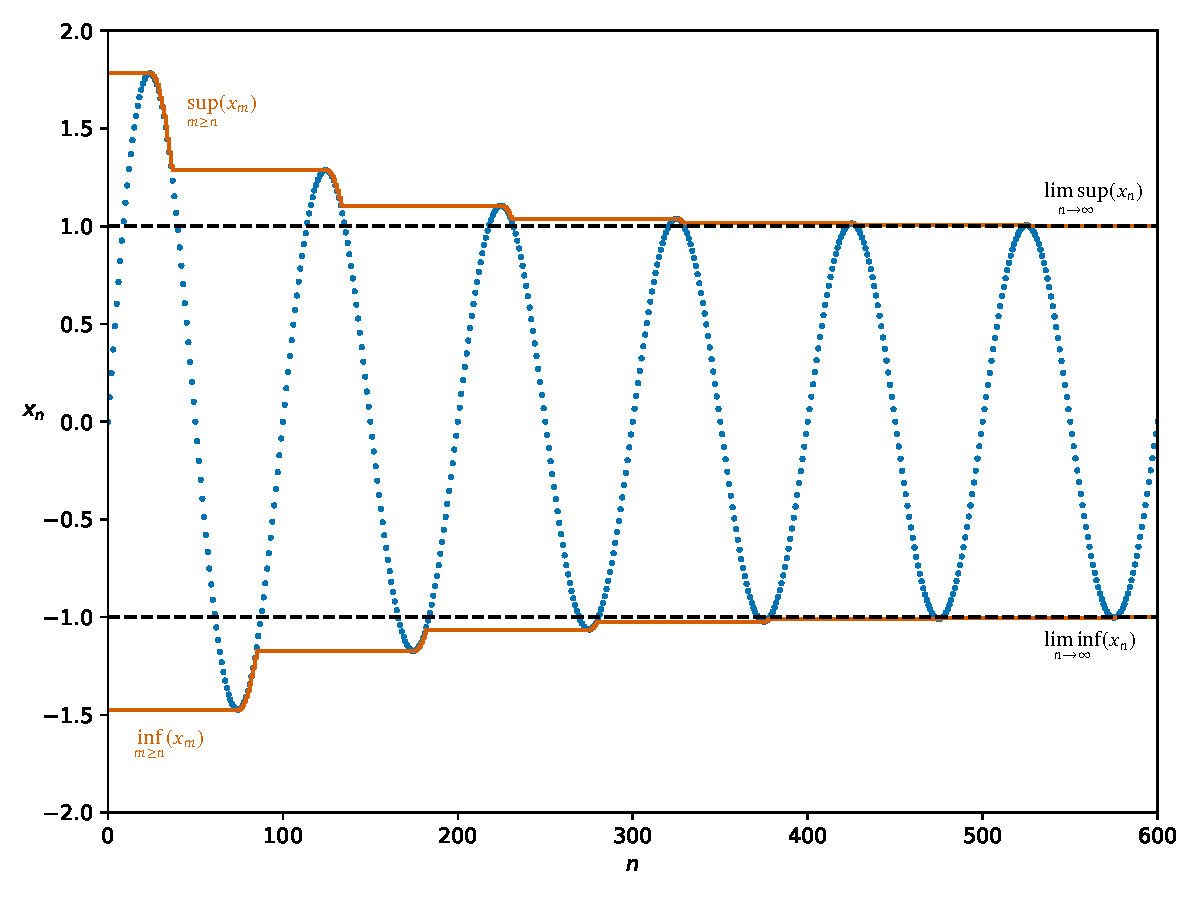
\includegraphics[width=1.0\textwidth]{ABSOLUTEPATH/pictures/light-mode/liminf-limsup/liminf-limsup.pdf}
    \end{webcompile}%
    Here:
    \begin{itemize}
        \item The sequence $(x_{n})_{n\in\N}$ is shown in \textcolor{OIblue}{blue}.
        \item The two \textcolor{OIvermillion}{orange} curves approach the limit superior and limit inferior of $(x_{n})_{n\in\N}$, shown as dashed black lines.
        \item The sequence accumulates around the two limits.
        \item The superior limit is the larger of the two, and the inferior limit is the smaller of the two.
        \item The inferior and superior limits agree \textiff the sequence is convergent (i.e., when there is a single limit).
    \end{itemize}
\end{remark}
\begin{proposition}{Properties of Sequences in $\R$}{properties-of-sequences-in-r}%
    Let $\smash{(x_{n})_{n\in\N}}$ and $\smash{(y_{n})_{n\in\N}}$ be sequences in $\R$.
    \begin{enumerate}
        \item\label{properties-of-sequences-in-r-characterisations-of-convergence}\SloganFont{Characterisations of Convergence. }The following conditions are equivalent:
            \begin{enumerate}
                \item The sequence $(x_{n})_{n\in\N}$ converges.
                \item We have%
                    %--- Begin Footnote ---%
                    \footnote{%
                        In this case, we have
                        \[
                            \limsup_{n\to\infty}(x_{n})
                            =
                            \lim_{n\to\infty}(x_{n})
                            =
                            \liminf_{n\to\infty}(x_{n}).
                        \]
                        \par\vspace*{-0.75\baselineskip}
                    }%
                    %---  End Footnote  ---%
                    \[
                        \limsup_{n\to\infty}(x_{n})
                        =
                        \liminf_{n\to\infty}(x_{n}).
                    \]%
            \end{enumerate}
        \item\label{properties-of-sequences-in-r-subtraction}\SloganFont{Subtraction. }We have
            \[
                \limsup_{n\to\infty}(-x_{n})
                =
                -\liminf_{n\to\infty}(x_{n}).
            \]%
        \item\label{properties-of-sequences-in-r-addition}\SloganFont{Addition. }We have%
            %--- Begin Footnote ---%
            \footnote{%
                The right hand sides of these should not be of the form $+\infty-\infty$ or $-\infty+\infty$.
            }%
            %---  End Footnote  ---%
            \begin{align*}
                \limsup_{n\to\infty}(x_{n}+y_{n}) &\leq \limsup_{n\to\infty}(x_{n})+\limsup_{n\to\infty}(y_{n}),\\
                \liminf_{n\to\infty}(x_{n}+y_{n}) &\geq \liminf_{n\to\infty}(x_{n})+\liminf_{n\to\infty}(y_{n}).
            \end{align*}
        \item\label{properties-of-sequences-in-r-multiplication-1}\SloganFont{Multiplication \rmI. }We have%
            %--- Begin Footnote ---%
            \footnote{%
                The right hand sides of these should not be of the form $0\cdot\infty$ or $\infty\cdot0$.
            }%
            %---  End Footnote  ---%
            \begin{align*}
                \limsup_{n\to\infty}(x_{n}y_{n}) &\leq (\limsup_{n\to\infty}(x_{n}))(\limsup_{n\to\infty}(y_{n})),\\
                \liminf_{n\to\infty}(x_{n}y_{n}) &\geq (\liminf_{n\to\infty}(x_{n}))(\liminf_{n\to\infty}(y_{n})).
            \end{align*}
        \item\label{properties-of-sequences-in-r-multiplication-2}\SloganFont{Multiplication \rmII. }If $\smash{\displaystyle\lim_{n\to\infty}(x_{n})}$ exists%
            %--- Begin Footnote ---%
            \footnote{%
                The case $A=\infty$ is allowed.
                \par\vspace*{-1.75\baselineskip}
            }, %
            %---  End Footnote  ---%
            then
            \[
                \limsup_{n\to\infty}(x_{n}y_{n})
                =
                \lim_{n\to\infty}(x_{n})%
                \limsup_{n\to\infty}(y_{n})
            \]%
            as long as the right hand side of the above equality is not of the form $0\cdot\infty$.
        %\item\label{properties-of-sequences-in-r-}\SloganFont{. }
        \item\label{properties-of-sequences-in-r-the-bolzano-weierstrass-theorem}\SloganFont{The Bolzano--Weierstrass Theorem. }Every bounded sequence in $\R$ has a convergent subsequence with limit in $\R$.
    \end{enumerate}
\end{proposition}
\begin{Proof}{Proof of \cref{properties-of-sequences-in-r}}%
    \FirstProofBox{\cref{properties-of-sequences-in-r-characterisations-of-convergence}: Characterisations of Convergence}%
    Omitted.

    \ProofBox{\cref{properties-of-sequences-in-r-subtraction}: Subtraction}%
    Omitted.

    \ProofBox{\cref{properties-of-sequences-in-r-addition}: Addition}%
    Omitted.

    \ProofBox{\cref{properties-of-sequences-in-r-multiplication-1}: Multiplication \rmI}%
    Omitted.

    \ProofBox{\cref{properties-of-sequences-in-r-multiplication-2}: Multiplication \rmII}%
    Omitted.

    \ProofBox{\cref{properties-of-sequences-in-r-the-bolzano-weierstrass-theorem}: The Bolzano--Weierstrass Theorem}%
    Omitted.
\end{Proof}
\begin{appendices}
\input{ABSOLUTEPATH/chapters2.tex}
\end{appendices}
\end{document}
